\chapter{Results and Discussion}
\label{chap:results}

This chapter gives an overview of the achieved results from all considered scenarios and cases.
The first section talks about a small network with only one user and one \gls{UAV}s. In 
the following section, this network is expanded for a larger population but still with one \gls{UAV}s.
The last section is also for a large population but with an unlimited number of \gls{UAV}s.

%%%%%%%%%%%%%%%%%%%%%%%%%%%%%%%%%%%%%%%%%%%%%%%%%%%%%%%%%%%%%%%%%%%%%%%%%%%%%%%%%%%%%%%%%%%%%%%%%%%%%%%%%%%%%%%%%%%%%%%%%%%%%%%%%%%%
\section{Scenario 1: One User and One \gls{UAV}}
The network contains only one user in this scenario. This means that there is only one location possible for the \gls{UAV} which will 
be just above 
the user. This section will investigate minimal required transmission power and SAR values from different sources.
Finally, also the power consumption of the entire network is measured. The  ``entire network" refers to all \gls{UABS}s. The entire network 
will for the first scenario be constructed out of a singe \gls{UABS}.

\subsection{The Influence of the Maximum Transmission Power}
\label{s1a}
\gls{LTE} makes usage of power control meaning that no more power will be used than strictly necessary. The actual 
transmission power $P_{tx}$ therefore ranges between zero and the maximum allowed input power. $P_{tx}$ is zero when the \gls{UABS} doesn't cover anybody.
For instance when the flying height is too high and therefore also the path loss that comes with it, the maximum allowed $P_{tx}$ is not enough to cover 
the distance. In such case, the \gls{UABS} is shut down since it cannot meet the requirements.
Increasing the maximum transmission power will not influence the actual used $P_{tx}$ or $SAR_{10g}$ because the \gls{UABS} will not use more
than strictly required. It is therefore more useful to match the actual transmission power against a variable flying height. 

Figure \ref{fig:ptxfh} shows a logarithmic relationship between $P_{tx}$ and flying height.
As already discussed in \ref{sec:scenarios_s1}, the user is outdoor and just below the \gls{UABS}. There is thus a free \gls{LOS} between both
radiators. It is clear from figure \ref{fig:ptxfh} that a discontinue step function is achieved. This is because multiple flying heights correspond to the same transmission power.
When the flying height increases, so does the path loss. \gls{LTE} tries to counteract this by increasing the power level. Each time 
the path loss becomes too high, the power level of the antenna increases with one dBm. Doing so, decreases path loss allowing the antenna to reach
the user again. 

\begin{figure}[t]
  \centering
  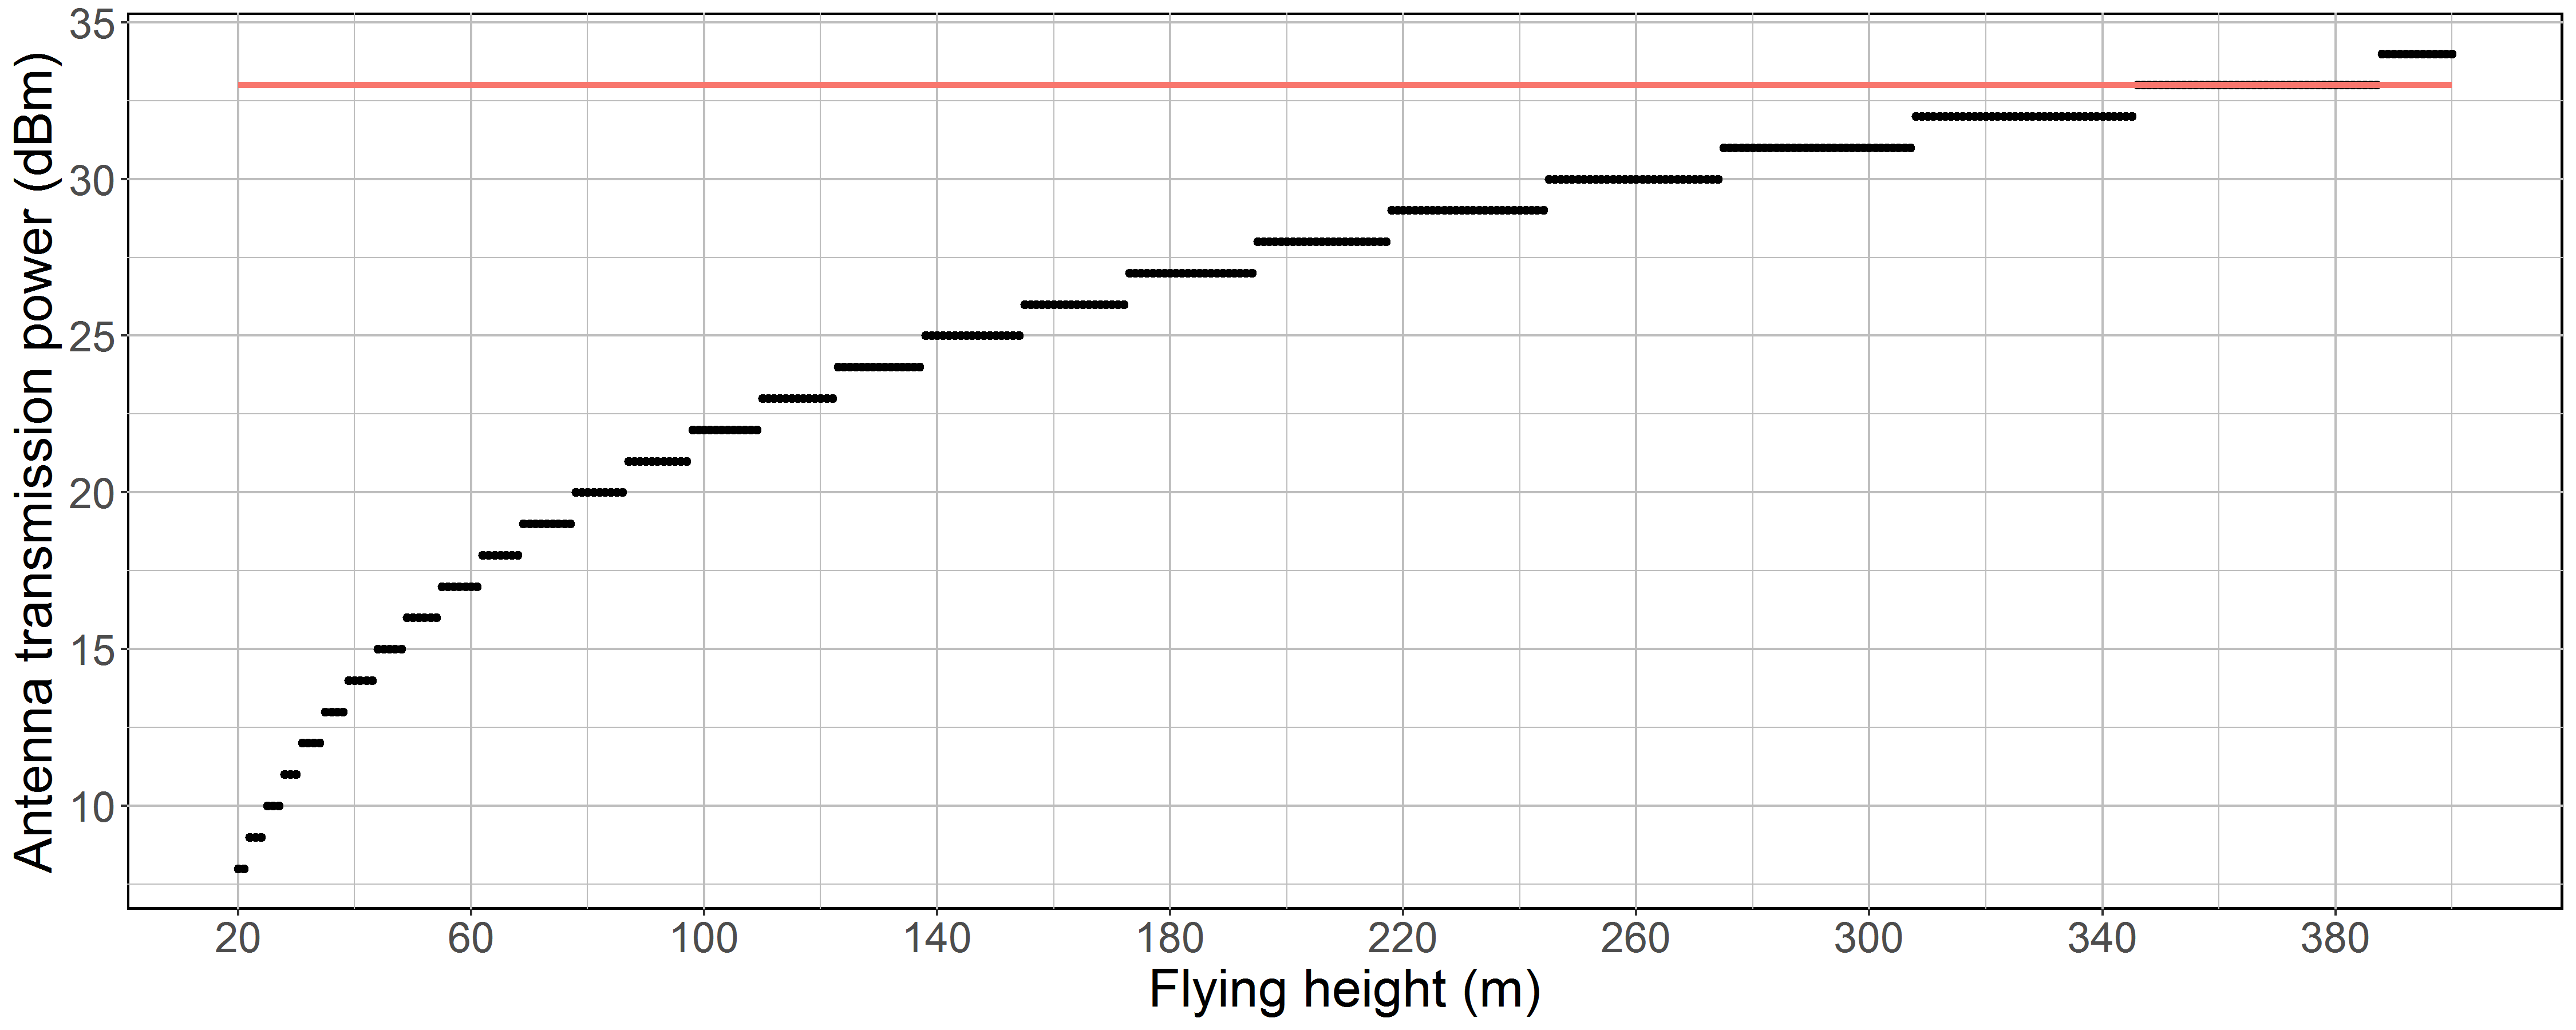
\includegraphics[width=\textwidth]{../results/s1/ptx.png}
  \caption{Minimal required transmission power by the antenna to reach the ground just below him. The red line shows the default maximum transmission power.}
  \label{fig:ptxfh}
\end{figure}

After a jump in the step function, there is an overestimation meaning the input power increased more than necessary. So multiple flying heights correspond with the same $P_{tx}$.
Further, dBm is also a logarithmic scale meaning that while 10 dBm equals 10 mW, 20 dBm equals 100 mW. This explains why the black lines become longer at higher flying altitudes.
Each time the power level increases with one dBm, the overestimation becomes larger. If the tool would make usage of a smaller step size, a more continuous 
logarithmic function would be achieved. This would however worsen the time complexity because it would take much more iterations before 
the power level exceeds the path loss. 

The red line in figure \ref{fig:ptxfh} indicates the default maximum transmission power used during simulations as 
defined in table \ref{table:defaultconf}. 
In a free line-of-sight scenario with only one user, a \gls{UABS} can fly up to 387 meters before losing connection.

This scenario is investigated with a microstrip patch antenna using power consumption optimization. 
 However, the chosen optimization strategy doesn't really matter as already explained in  \ref{sec:scenarios_s1}. This is because the decision 
 algorithm decides which user 
needs to be connected to which \gls{UABS}. Since only one \gls{UABS} is available, both optimization strategies will behave identical.
Further, also the used antenna will not make any difference
despite the fact that a microstrip patch antenna has attenuation while an \gls{isotropicradiator} doesn't.
The user is namely positioned in the perfect center of the main beam where there is 
no attenuation experienced in either cases. So the results are applicable for the four possible cases from figure \ref{fig:fourCasesMatrix}.

\FloatBarrier
\subsection{Influence of the Flying Height}
\label{sub:senario1_influenceOfFlyHeight}

This section investigates how the flying height of a \gls{UABS} influences $SAR_{10g}$ and power consumption.
The $SAR_{10g}$, which is actually induced electromagnetic radiation into our user, is represented in figure \ref{fig:s1_fhsar}
and shows that for a low flying \gls{UAV}, \gls{DL} radiation is the main source of electromagnetic exposure.
This changes around 80 meters where the \gls{UL} radiation from the \gls{UE}
exceeds the \gls{DL} radiation in order to still be able to reach the high flying \gls{UABS}s.

\gls{SAR}-values are caused by the transmitted power  $P_{tx}$ of the antenna. The $P_{tx}$ in section \ref{s1a}
showed a discontinue behaviour that sometimes radiates more as strictly necessary. This has thus a direct influence
on the \gls{DL} \gls{SAR}. Hence the same discontinue behaviour. The \gls{DL} \gls{SAR} can be simplified to a perfect constant line.
This constant behaviour can once again be explained with power control. When the \gls{UABS} flies lower, there is less path loss and the \gls{UABS} 
will therefore reduce the $P_{tx}$. This results in formula \ref{eq:exposureBasicFormula} where the electromagnetic exposure is a constant fraction of power and distance.

\begin{equation}
\vec{E} (V/m) = \frac{\Delta U (V) }{\Delta x (m)}
\label{eq:exposureBasicFormula}
\end{equation}

%The SAR values are the result of multiplying the electromagnetic exposure with a constant as explained in equation \ref{eq:DLconvertion}. So both have a linear relationship.

Figure \ref{fig:s1_fhsar} doesn't show radiation from neighbours, because there are none present in this scenario. 
Finally, all these values are added up as explained in formula \ref{eq:overallSARwb} resulting in the total \gls{SAR}
to which our user is exposed which is represented by the black line in \ref{fig:s1_fhsar}.

\begin{figure}[]
  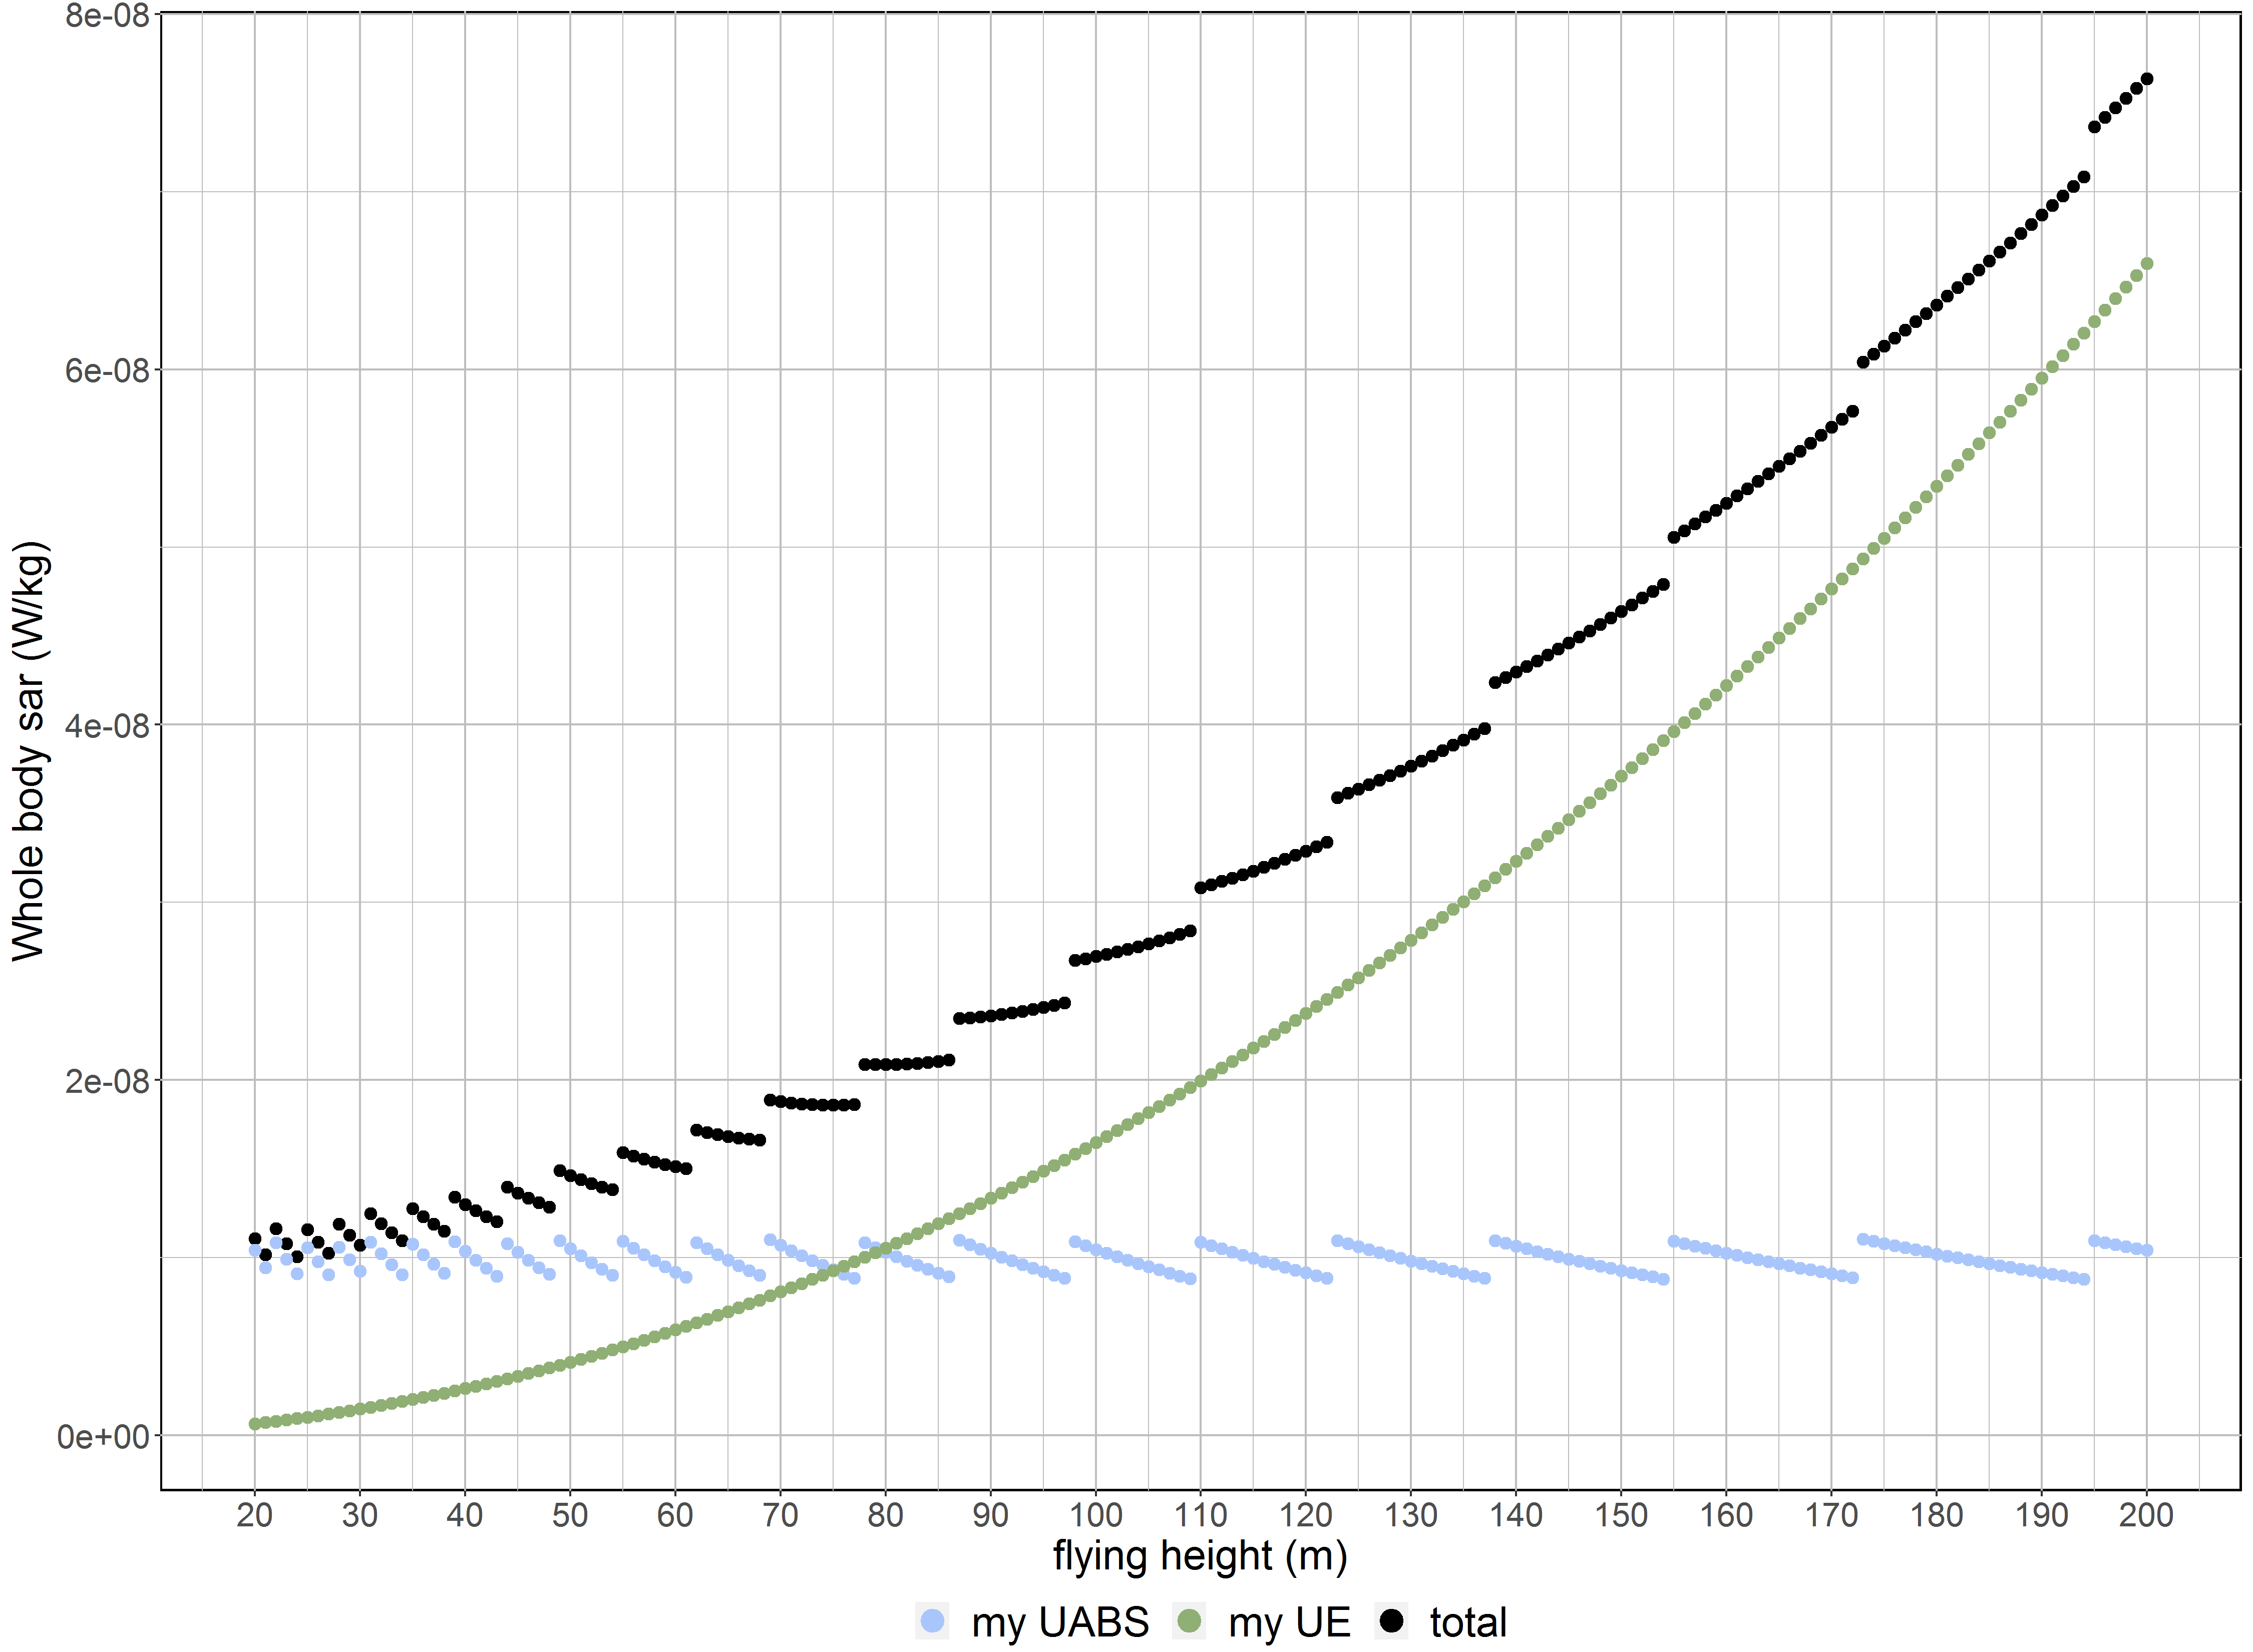
\includegraphics[width=\textwidth]{../results/s1/fhvssar.png}
  \caption{This figure showss how SAR values from different sources are influenced by different flying altitudes.}
  \label{fig:s1_fhsar}
\end{figure}

The power consumption of the entire network includes both the power required by the \gls{UAV} itself and the antenna he is carrying.
The power consumption of the entire network is here of course for the only \gls{UABS} available. Figure \ref{fig:fhvspc} shows an 
exponential relationship between both power consumption and flying height. This  is mainly caused by the antenna 
attached to the \gls{UABS} which will require more energy to maintain the same exposure on the ground but over a larger distance.

\begin{figure}[t]
  \centering
  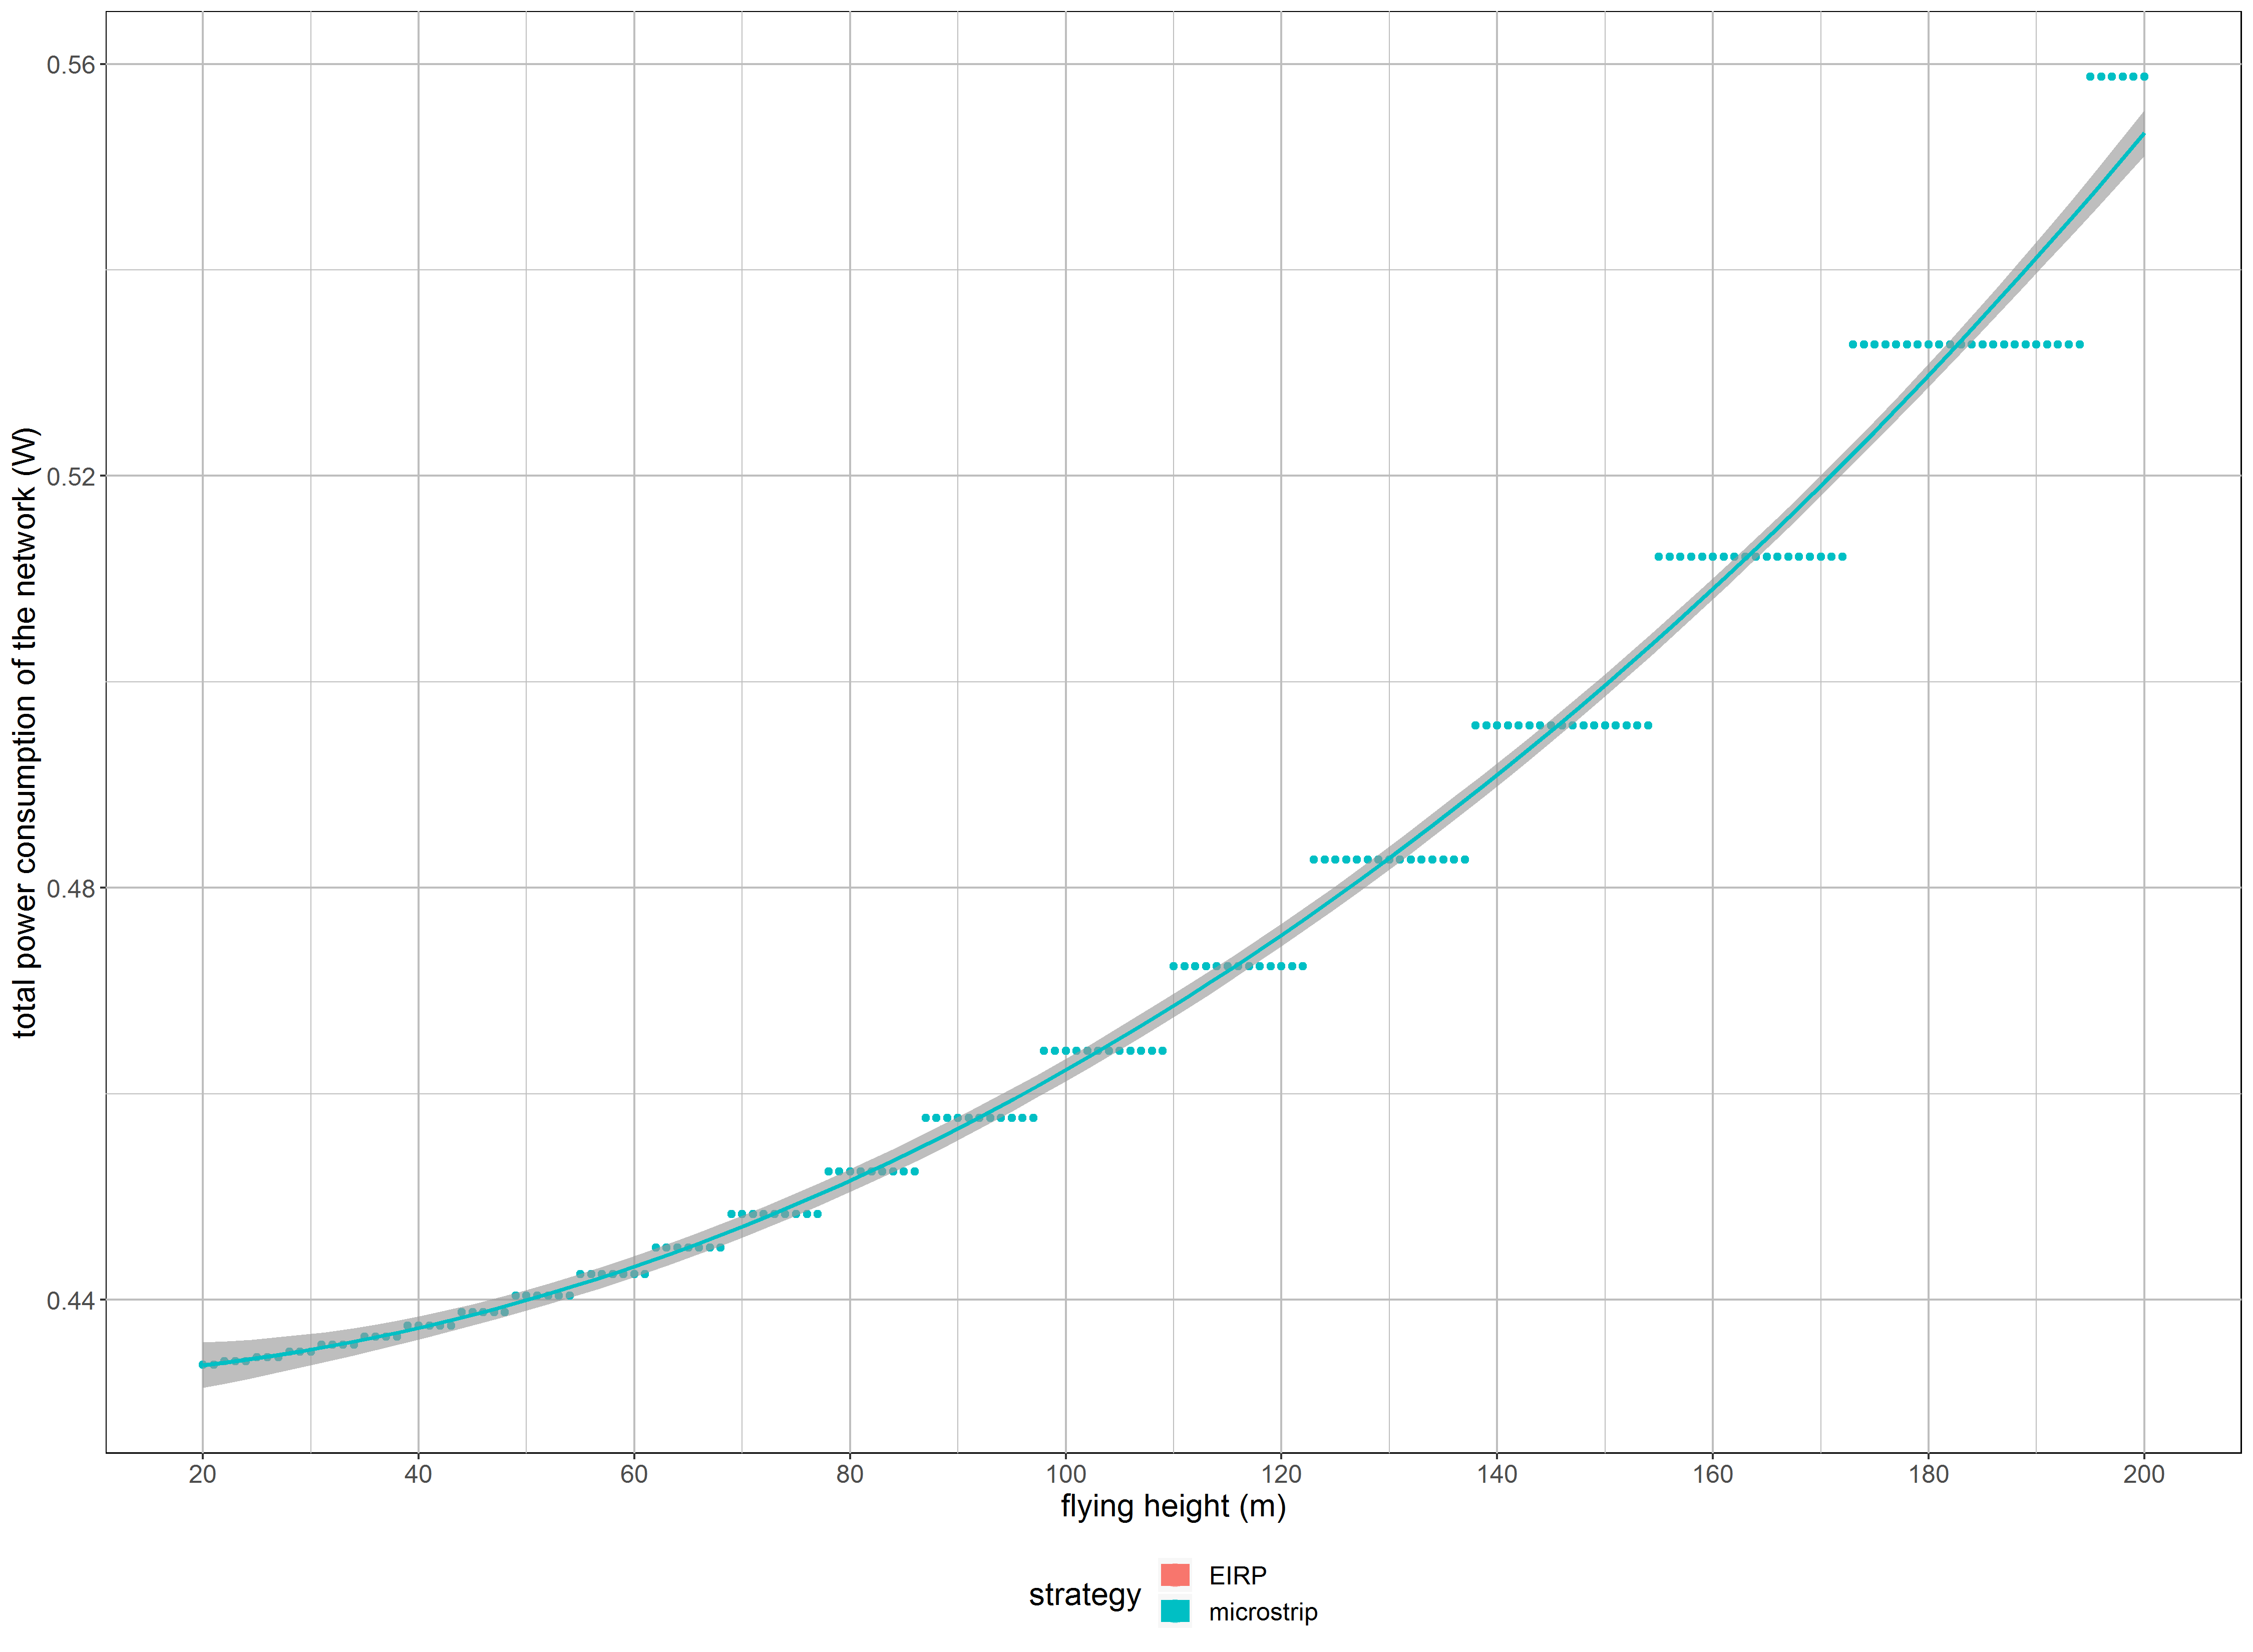
\includegraphics[width=\textwidth]{../results/s1/fhvspc.png}
  \caption{This figure shows the behaviour of the power consumption over the entire network at different flying  heights.
  For this scenario, this will only be one \gls{UABS}.}
  \label{fig:fhvspc}
\end{figure}

%%%%%%%%%%%%%%%%%%%%%%%%%%%%%%%%%%%%%%%%%%%%%%%%%%%%%%%%%%%%%%%%%%%%%%%%%%%%%%%%%%%%%%%%%%%%%%%%%%%%%%%%%%%%%
\FloatBarrier
\section{Scenario 2: Increased Traffic}

This scenario has just like the previous scenario only one \gls{UAV} available. However, more users will be present in the network.
First, a variable flying altitude is investigated for a fixed number of 224 users. 
Secondly, the flying height is set to 100 meters with a variable number of users.
When designing the network, there will be as much possible \gls{UAV} locations as there are users in the network and the tool
will consider all of them. It's only when the program is finished, that one \gls{UAV} will remain.

\subsection{Influence of the Flying Altitude}
The first case investigates how the network, consisting out of one \gls{UABS}, behaves when applied on an ordinary day during rush hours. 
Different fixed flying heights are considered while 224 active users are distributed uniformly over the city centre of Ghent. 

A power consumption optimized network with an \gls{EIRP} antenna (green) has the highest exposure. 
This is logical when comparing with an EIRP antenna in an exposure optimized network (red). 
However, when looking at figure \ref{fig:s2a_dlAndPc} on the right, the power consumption in a power consumption optimized network is worse 
than in an exposure optimized network. To understand this, the behaviour of the deployment tool needs to be understood first. 
A power consumption optimized network will result in a few high powered \gls{UABS}s because increasing the input power of an antenna costs 
less than activating a new  \gls{UAV}. Likewise, an exposure optimized network 
generates a lot of low powered \gls{UABS}s because the lower the power of the antenna, the lower the exposure. This has the consequence that the cover radius 
is less and therefore requires more \gls{UAV}s which costs more energy.
When only a limited amount of \gls{UABS}s are available, 
like only one in this scenario, the tool will only keep \gls{UABS}s which cover the most users. 
Therefore, the power consumption in a power consumption optimized network is much more higher. 


\begin{figure}[h!]
  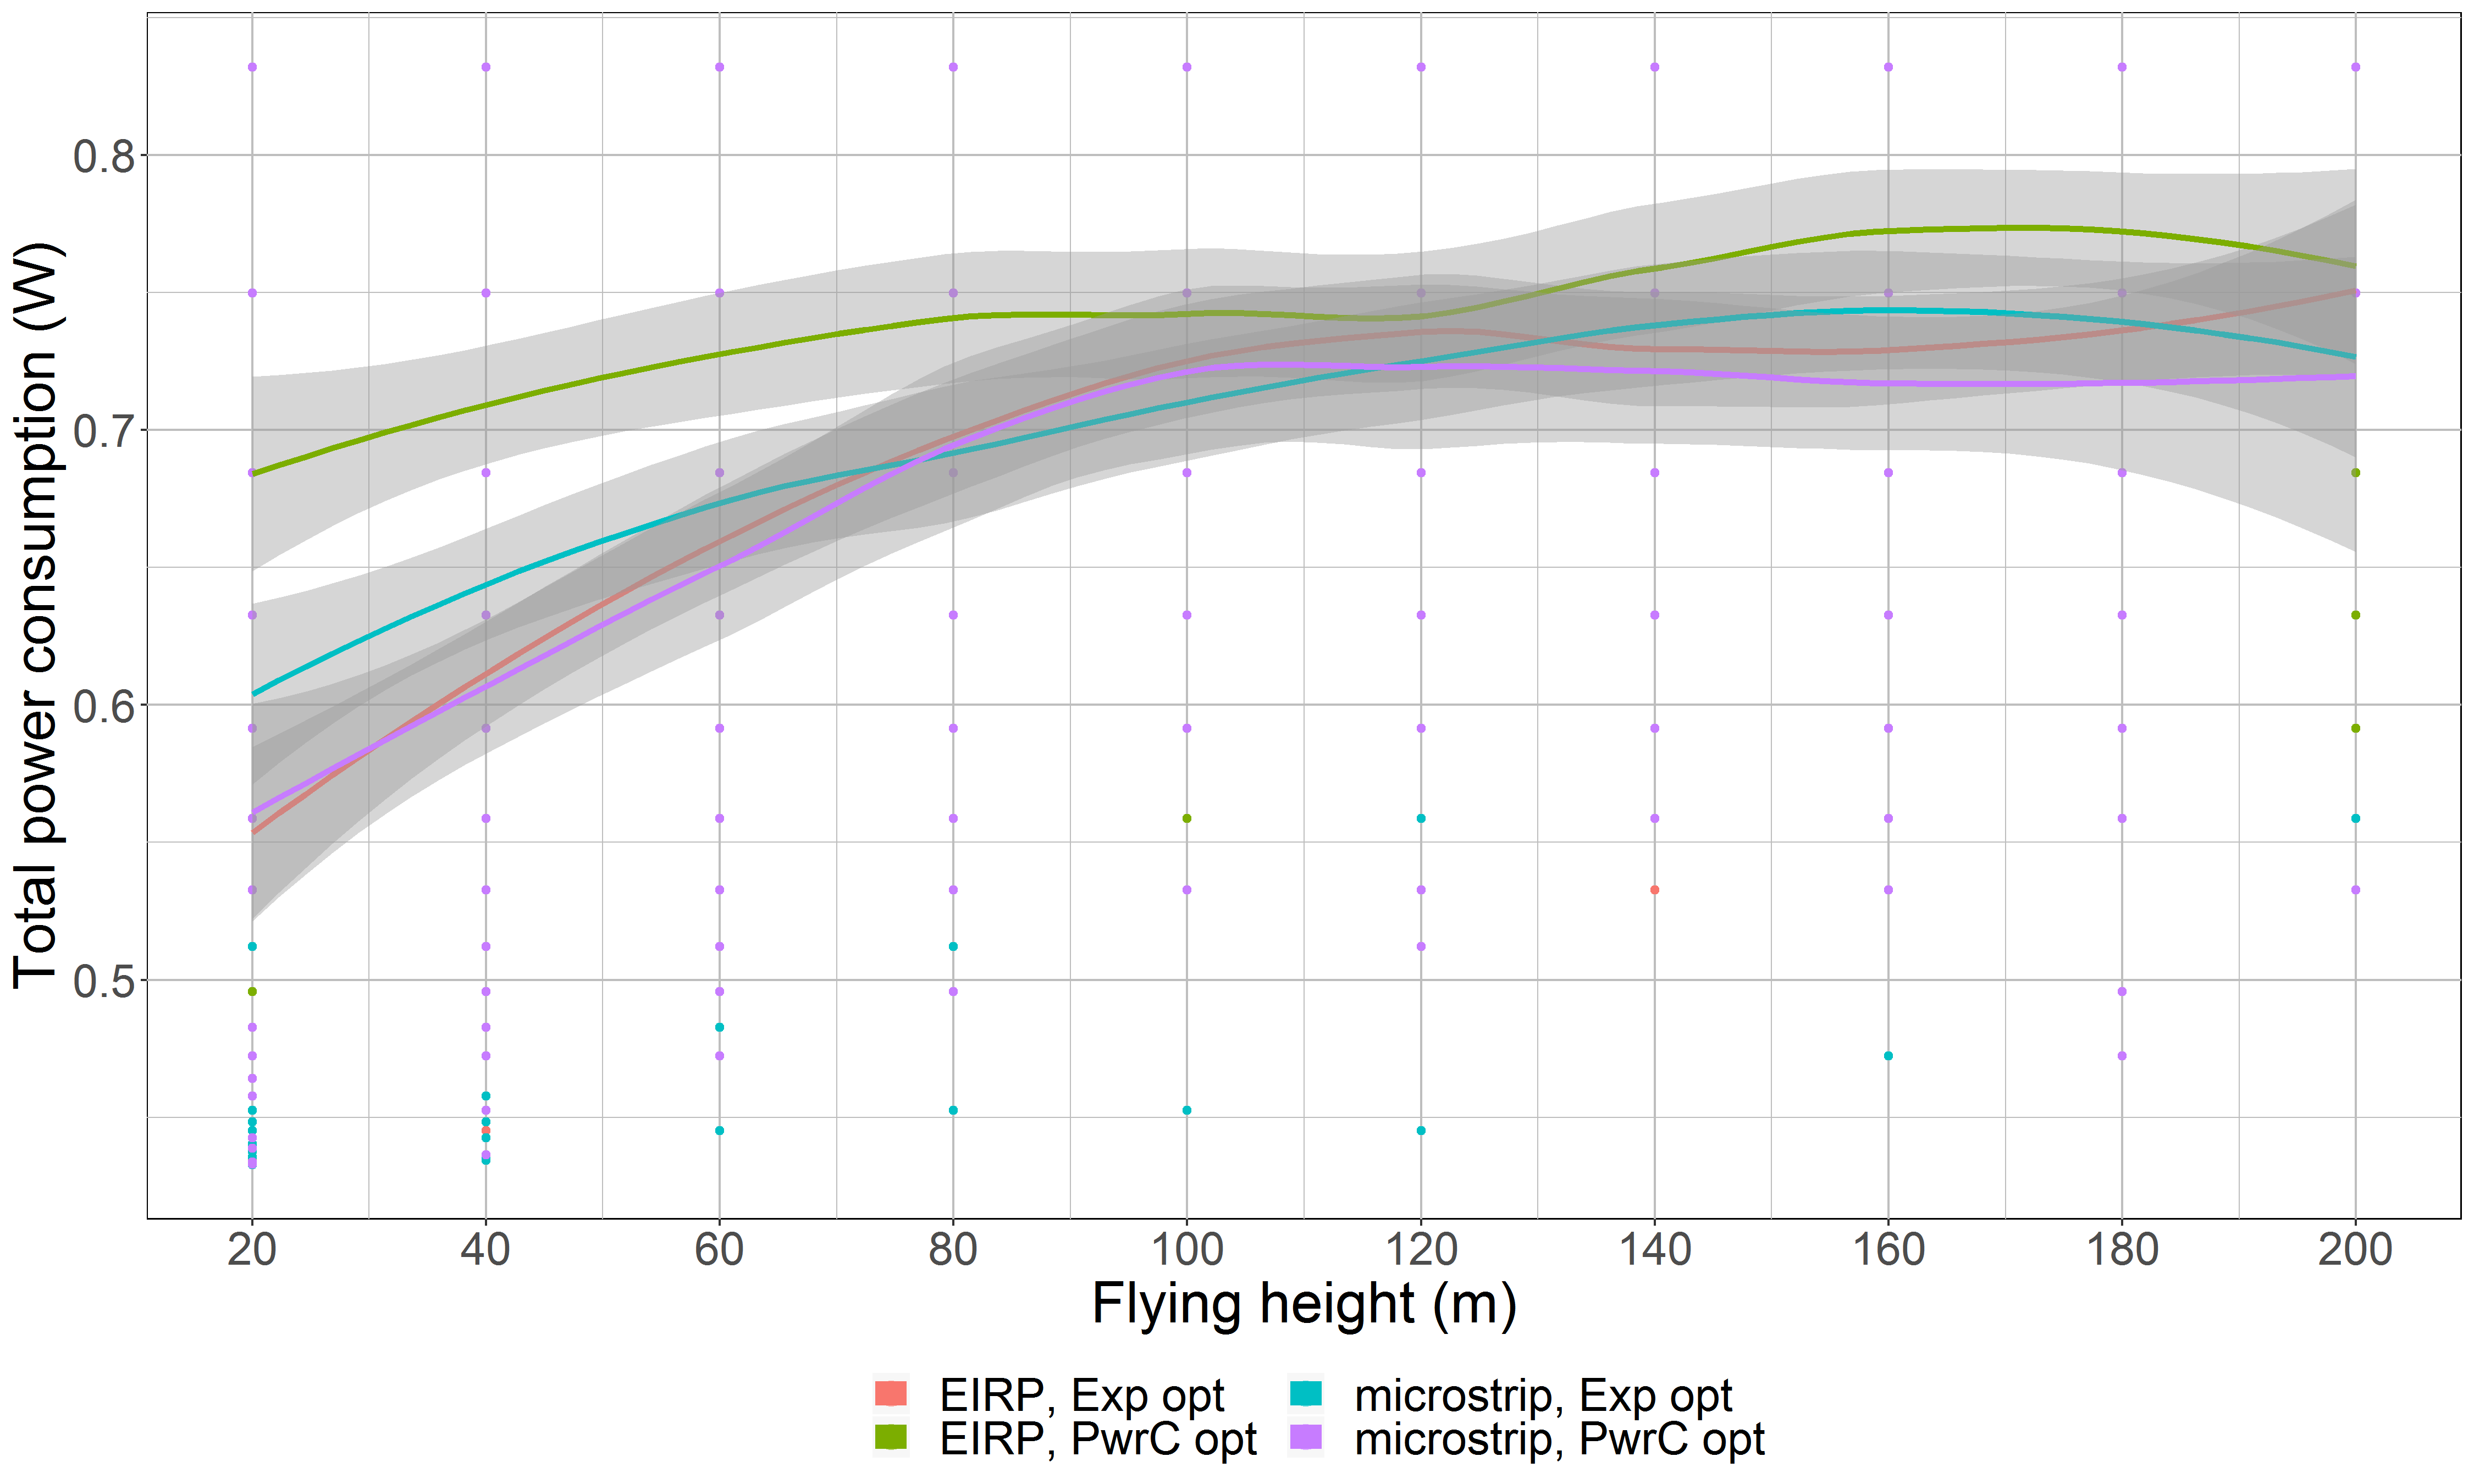
\includegraphics[width=\textwidth]{../results/s2/fhvsdlAndPc.png}
  \caption{These two figures show how the flying height influences the downlink electromagnetic radiation of the average user (left) and 
  power consumption of the entire network (rights) for one \gls{UABS} available in the network.}
  \label{fig:s2a_dlAndPc}
\end{figure}

The \gls{DL} exposure in figure \ref{fig:s2a_dlAndPc} increases along with the flying height. One might expect a more constant 
behaviour like it was the case in figure \ref{fig:s1_fhsar} of scenario 1. To understand this, the scenario has been reduced  
to only two users and is illustrated in figure \ref{fig:schematicprove}.
The two users, who will be referred to by `red' and `blue', are 90 meters separated from each other with a building between them.
Scenario 1 already explained that the charts can be simplified and the blue line from fig. \ref{fig:prove} remains in fact constant between the zero and 130 meters.
The chart shows that the \gls{UABS} is positioned above the blue user. The red user is in \gls{NLOS} as long as the \gls{UABS} remains below 20 meters.

\begin{figure}[]
  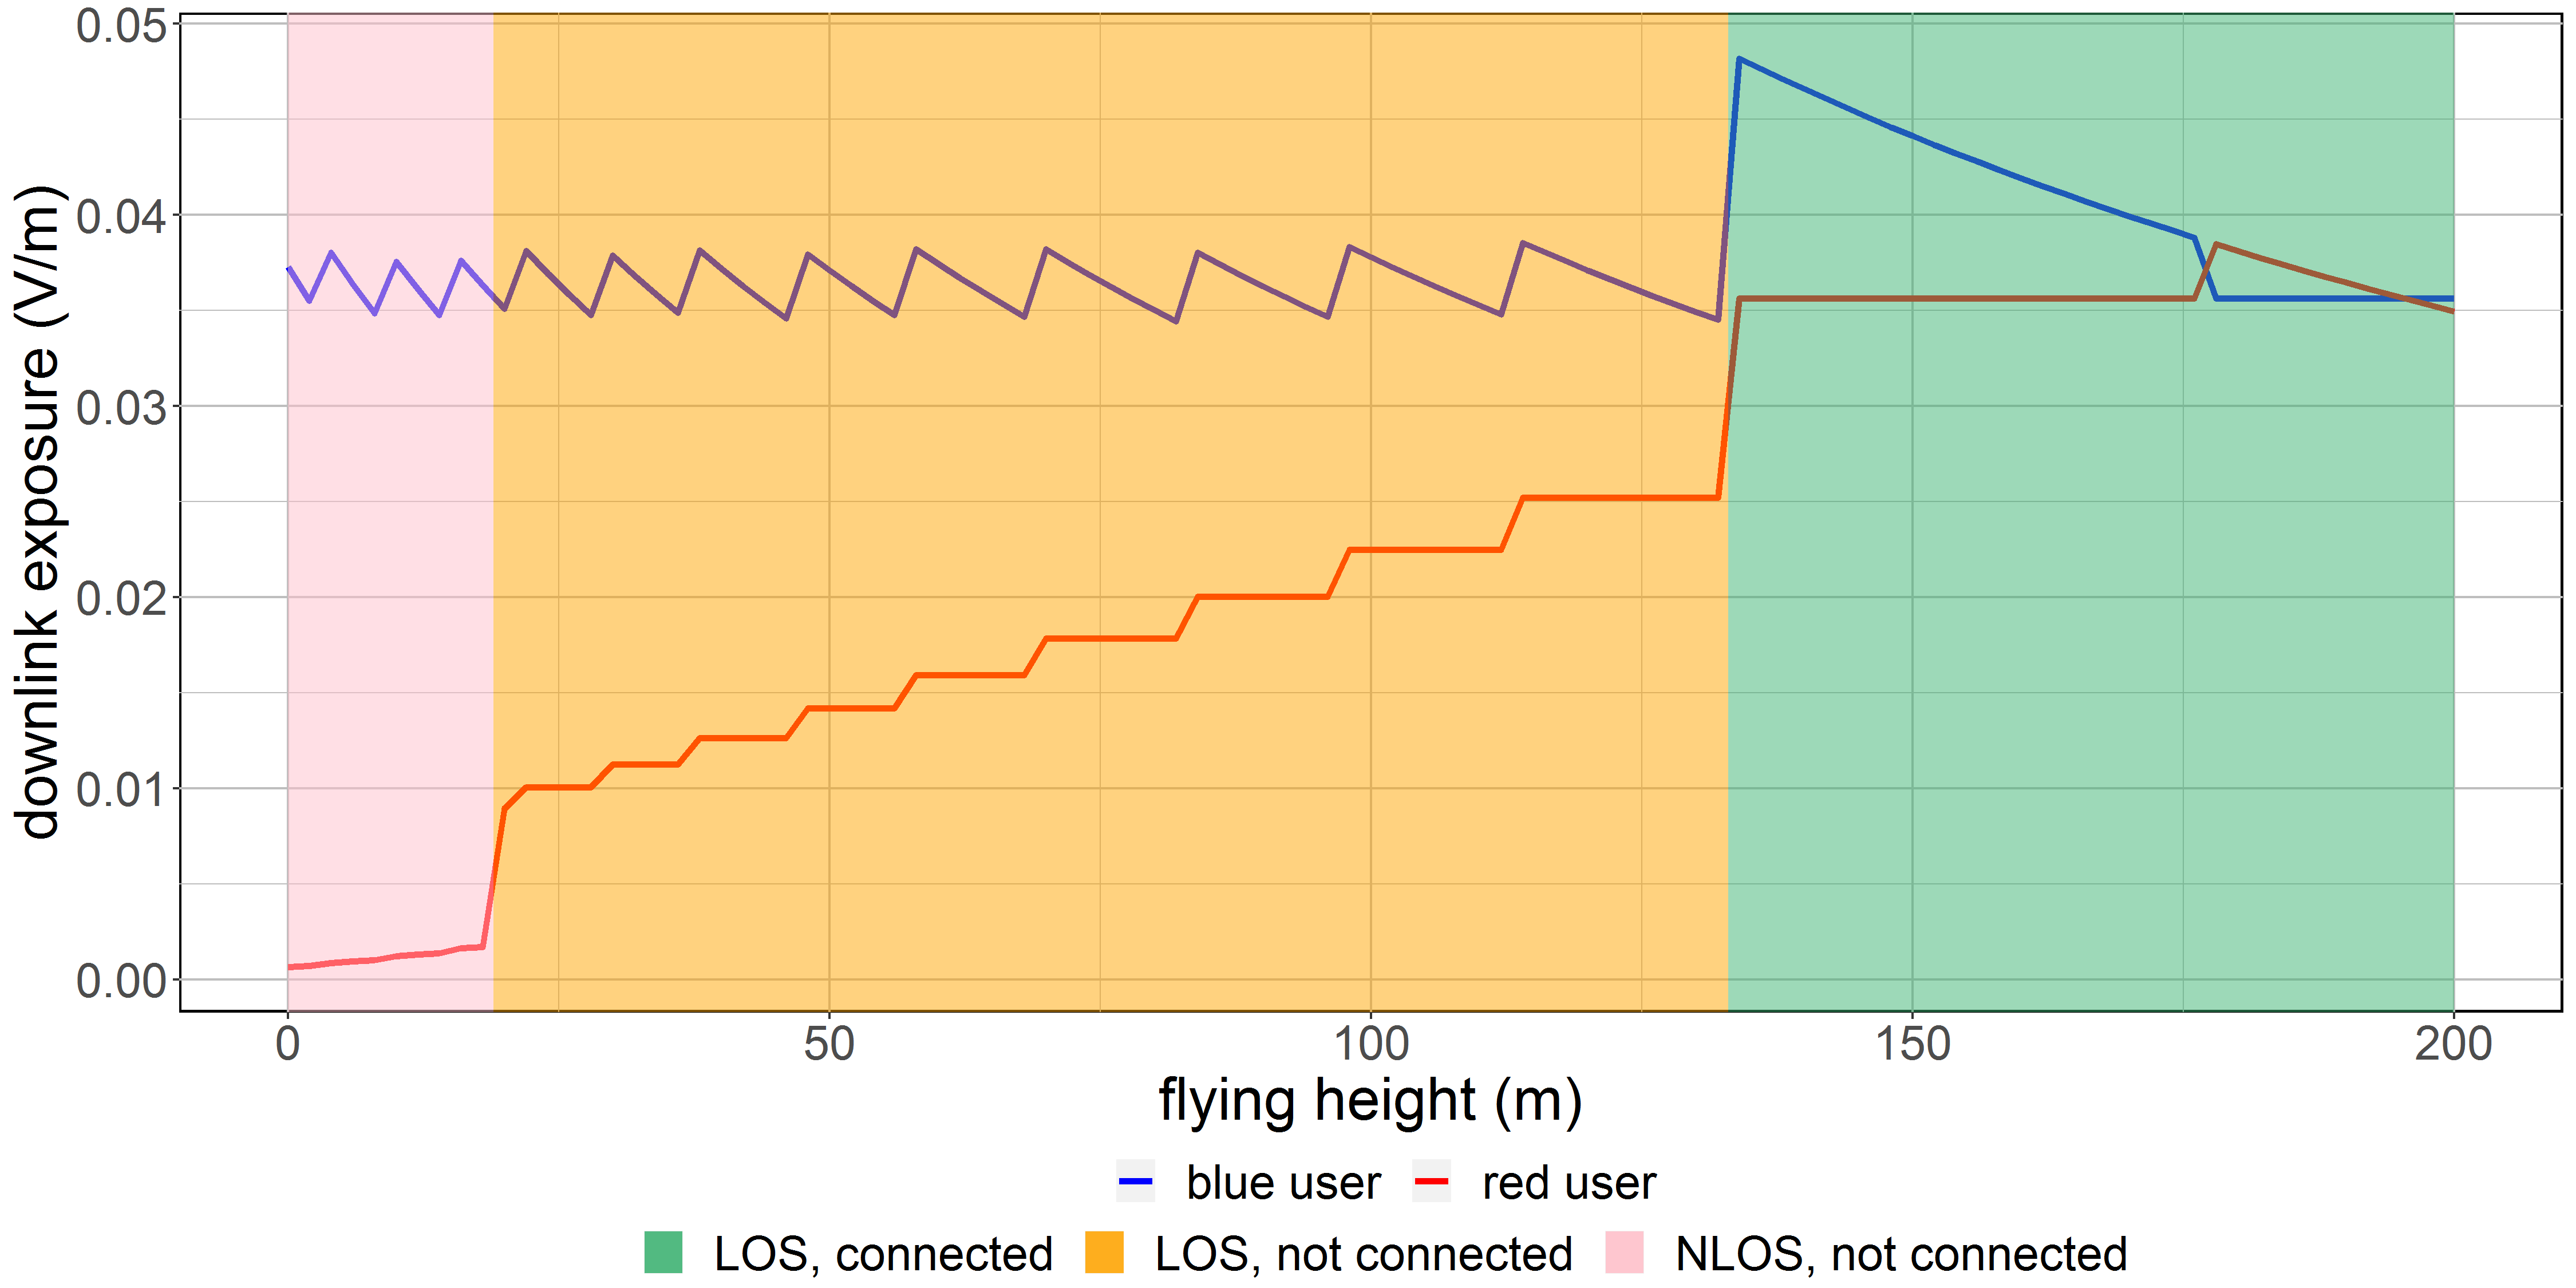
\includegraphics[width=\textwidth]{../results/s2/prove.png}
  \caption{Scenario 2 with only 2 users. The coloured areas are only applicable for the red user. The blue user is connected during the entire time.}
  \label{fig:prove}
\end{figure}


\begin{wrapfigure}{r}{0.48\textwidth}
  \begin{center}
    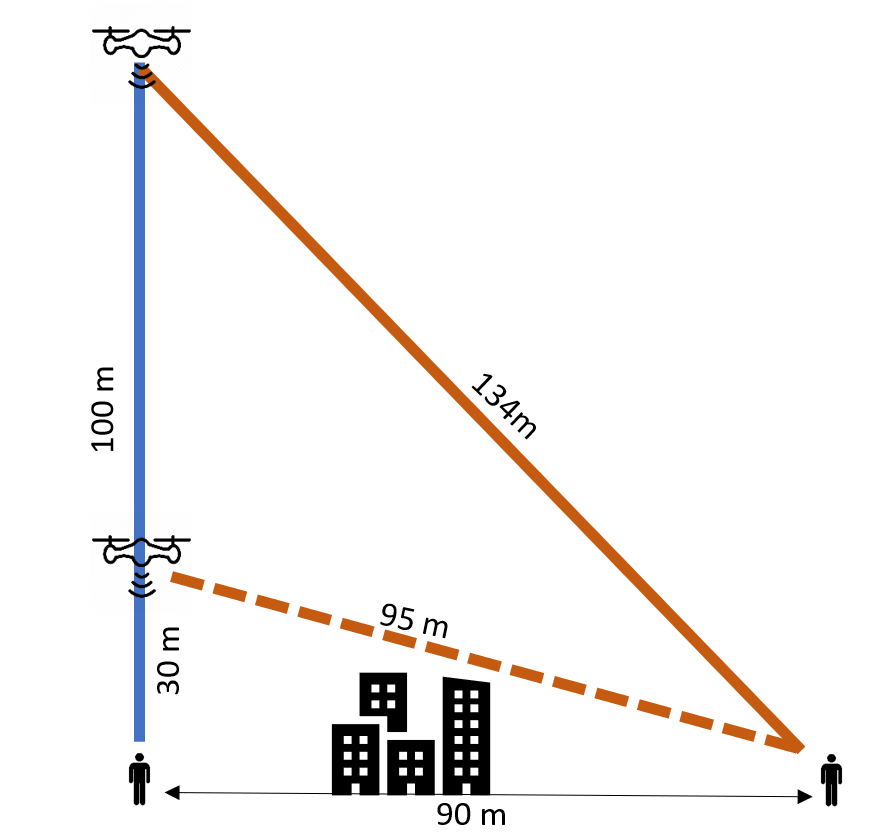
\includegraphics[width=0.48\textwidth]{../results/s2/proveScenario.png}
  \end{center}
  \caption{Schematic overview of scenario 2 with only 2 users.}
  \label{fig:schematicprove}
\end{wrapfigure}
Once the \gls{UABS} increases its flying altitude, the red user becomes into \gls{LOS} but still remains uncovered. This is because the tool initially locates a possible 
\gls{UABS} above each user and thereafter performs the  fitness function. The applied fitness function must have decided that it is better to connect 
each user to the \gls{UABS} above him. In a final stage, the tool checks whether the number of online \gls{UAV}s does not exceed the capacity of the facility
which is here the case. The tool therefore deactivates one \gls{UABS} causing the red user to be uncovered. One could argue that the 
the red user should be connected to the online \gls{UAV} who is only 90 meters away. This would however require the online \gls{UAV} to increase his power consumption which 
would make the decisions made by the optimization strategy obsolete.
When the \gls{UAV} flies higher, the difference in distance between both users and the base station decreases. In other words, the Pythagorean theorem shows that when the flying height of the 
\gls{UABS} increases, the distance with the blue user increases faster compared to the distance between that same \gls{UABS} and the red user. This is also illustrated in 
figure \ref{fig:schematicprove}.
At 130 meters, the tool decides to connect both users to the same \gls{UABS}. Therefore, it increases its power consumption whereby the red user would  have the minimal 
required electromagnetic exposure. This has of course a negative influence on the blue user who is much more closer and experiences now a much higher exposure level in fig \ref{fig:prove}.
Around 180 meters, the  red and blue line switch because the \gls{UAV} changes position. As explained before, the tool assigns two possible \gls{UAV}s, one above 
each user. The tool must have decided that connecting both users to the other \gls{UAV}s improves the fitness function of the entire network even though that difference might be 
very little. \\
Finally, this brings us back to the weighted average exposure from figure \ref{fig:s2a_dlAndPc} where 223 users will behave like the  red user and only
one user behaves like the blue one. 
The red line therefore dominates the average exposure in figure \ref{fig:s2a_dlAndPc}.

\begin{figure}[h]
  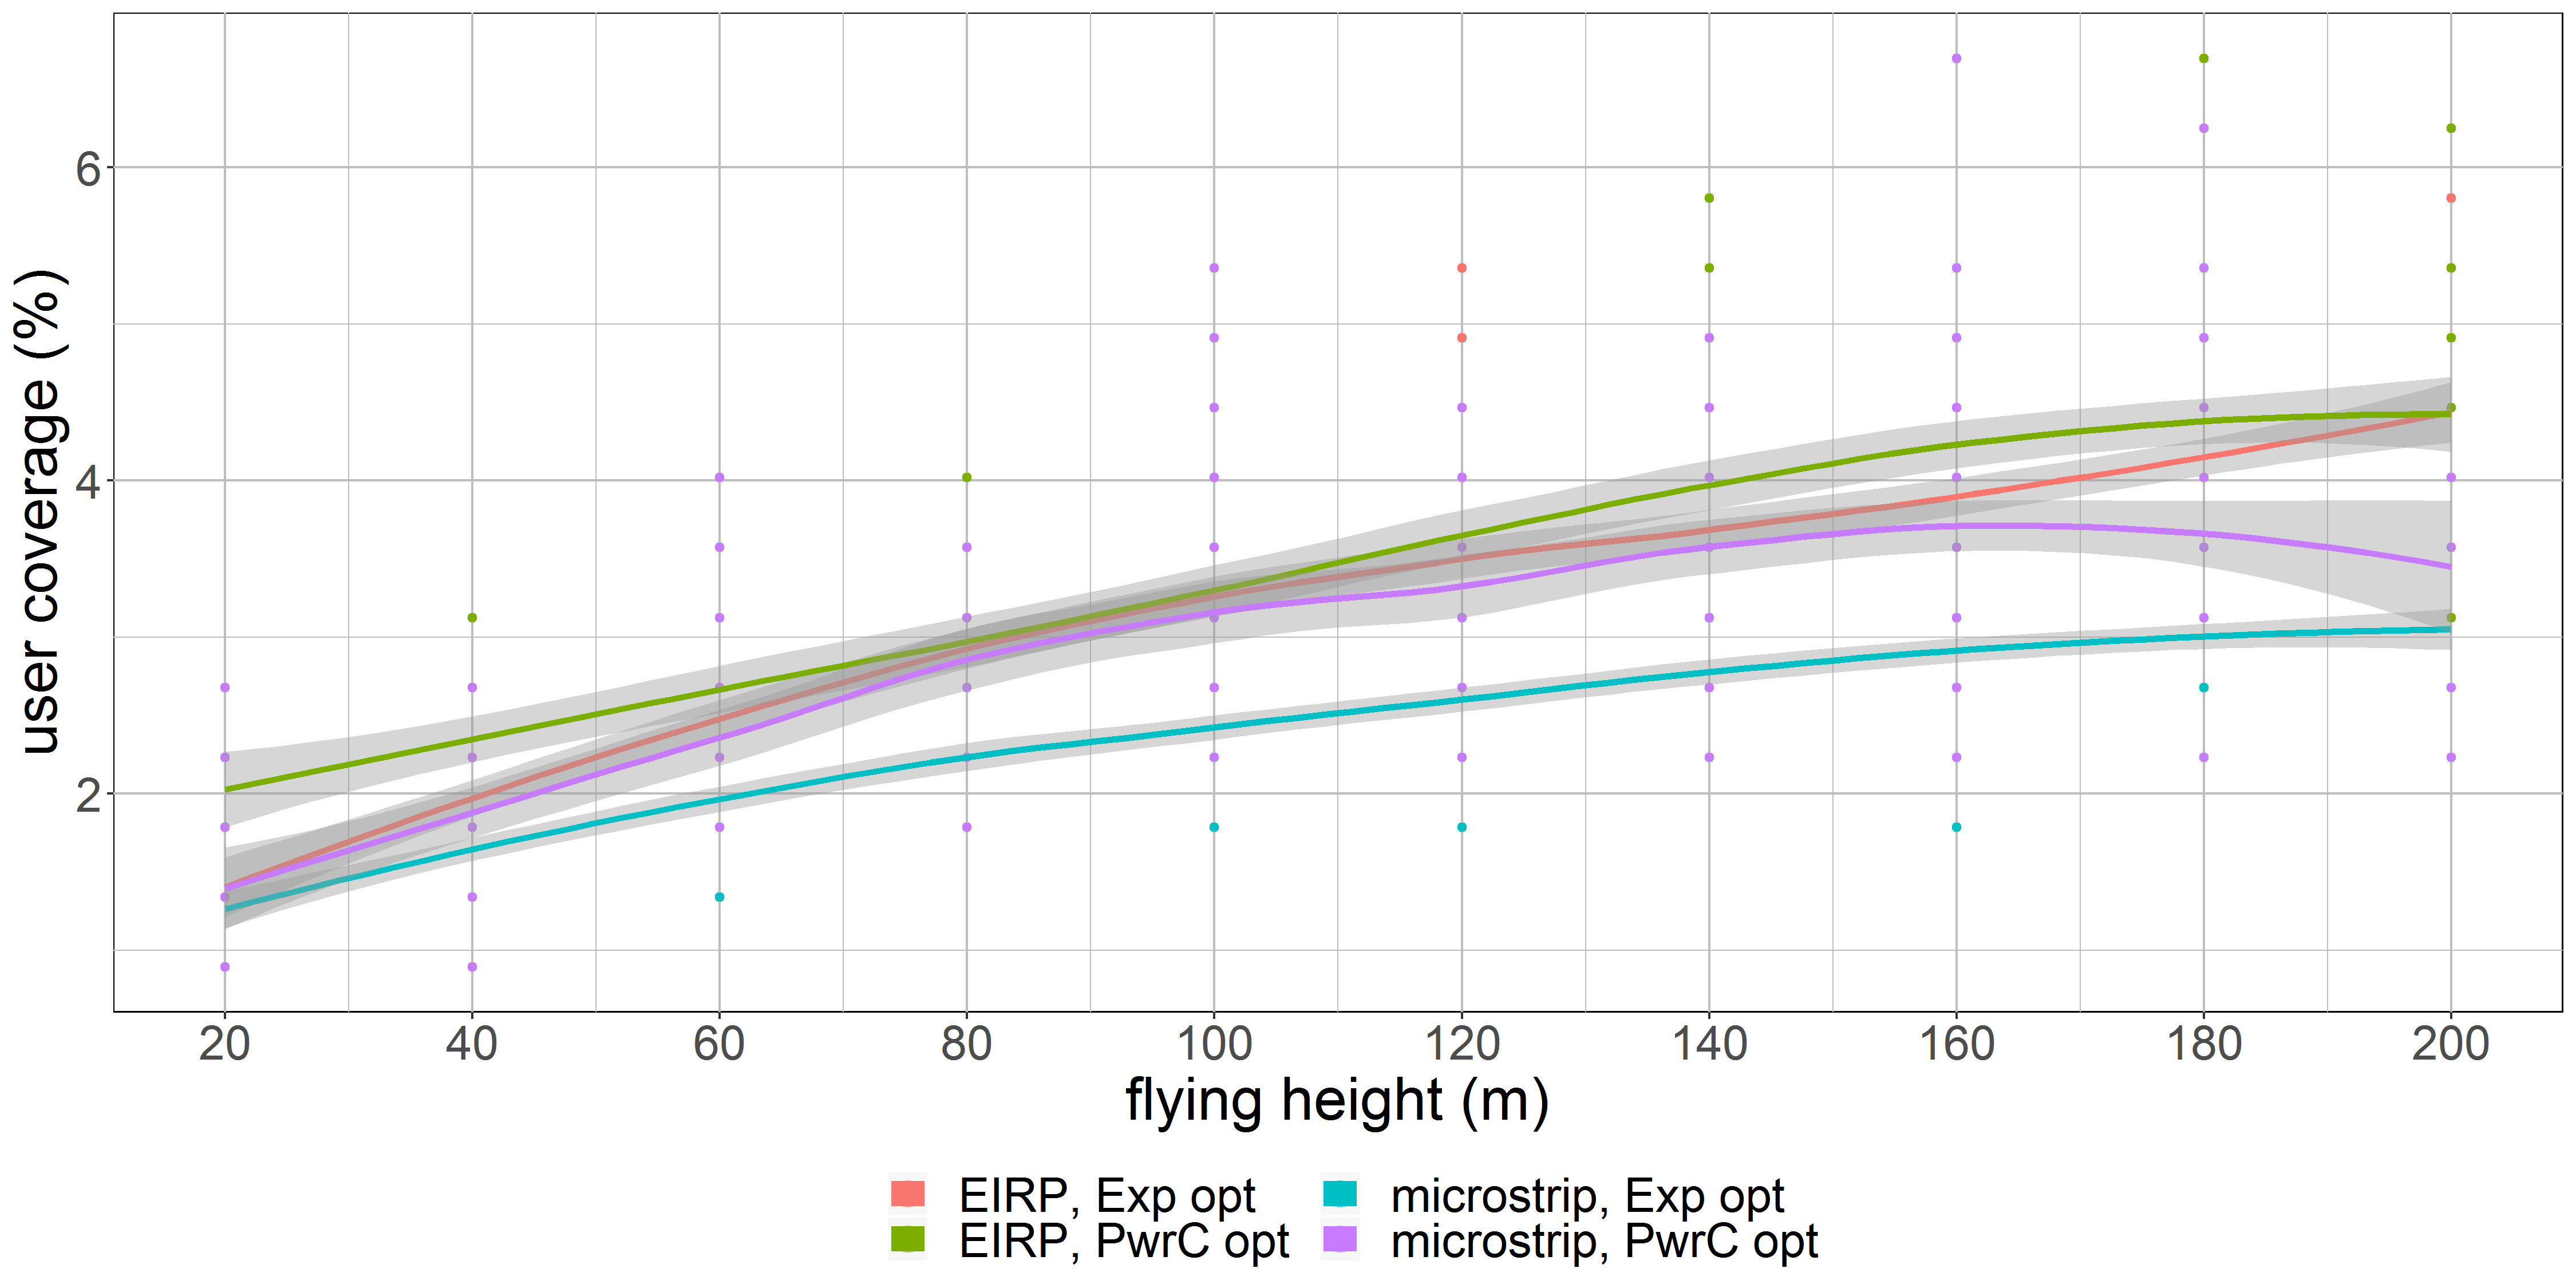
\includegraphics[width=\textwidth]{../results/s2/fhvscov.png}
  \caption{This graph shows the percentage of covered users for only one \gls{UABS} at different flying heights.}
  \label{fig:s2fhvscov}
\end{figure}

Figure  \ref{fig:s2fhvscov} shows that the flying height has a positive influence on the user coverage. 
When a \gls{UABS} flies higher, there is less path loss between the user and the \gls{UAV} caused by buildings but also the path loss to neighbouring 
users decreases as explained 
in figure \ref{fig:prove} and \ref{fig:schematicprove}. 
Also the increasing \gls{DL} exposure  from figure \ref{fig:s2a_dlAndPc}, from earlier, indicated that the
user coverage should grow. 
Figure \ref{fig:s2a_dlAndPc} further also shows how the \gls{SAR} from the \gls{UABS}
starts  decreasing again at high altitude. This is  not caused by the obstructing buildings but of the 
distance in general which becomes to high.  When this decrease happens depends on the configuration.  An power consumption optimized 
network tend to decrease earlier then an exposure optimized network.


When replacing the fictional \gls{EIRP} antenna by a microstrip patch antenna, the percentage of covered users drops for both 
optimization strategies. This is because users, who have a higher horizontal distance between themselves and the \gls{UABS}, 
experience a higher attenuation. When a microstrip patch antenna is positioned higher, the range of the antenna increases 
since the angle between the user and the \gls{UABS}s main lob decreases. The user will therefore experience less attenuation.

Eventually, figure \ref{fig:s2shfourSourcesMatrix} shows the total whole body $SAR_{10g}$ deducted from all electromagnetic sources. This being the exposure 
of the only \gls{UABS} available in the network, 
 the \gls{UL} exposure from the user’s own device and the exposure of the devices from all other users. 
 Thereafter, the weighted average whole body \gls{SAR} for each individual source in the network is calculated with the 50th and 95th percentile 
 being the most important values. This is because not only the mean value is important but also users who experience higher 
 levels of whole body $SAR_{10g}$.

When investigating the three different sources of which the total \gls{SAR}-values are based on, we see 
that the radiation from the \gls{UABS} is the main factor followed by the near-field radiation from the user's own device.
The far-field radiation from other \gls{UE} have barely influence. 
It looks like it is zero but it is just very low compared to the other two values and in fact increases when the flying height becomes larger.

The weighted average $SAR^{ul}_{10g}$ from the own device is zero in an exposure optimized network with a microstrip patch antenna which is even lower than the $SAR^{neighbours}_{10g}$.
This is because the coverage in this scenario is so low that the weighted average only consists of uncovered users and an uncovered user his device has no power consumption.

\begin{figure}[]
  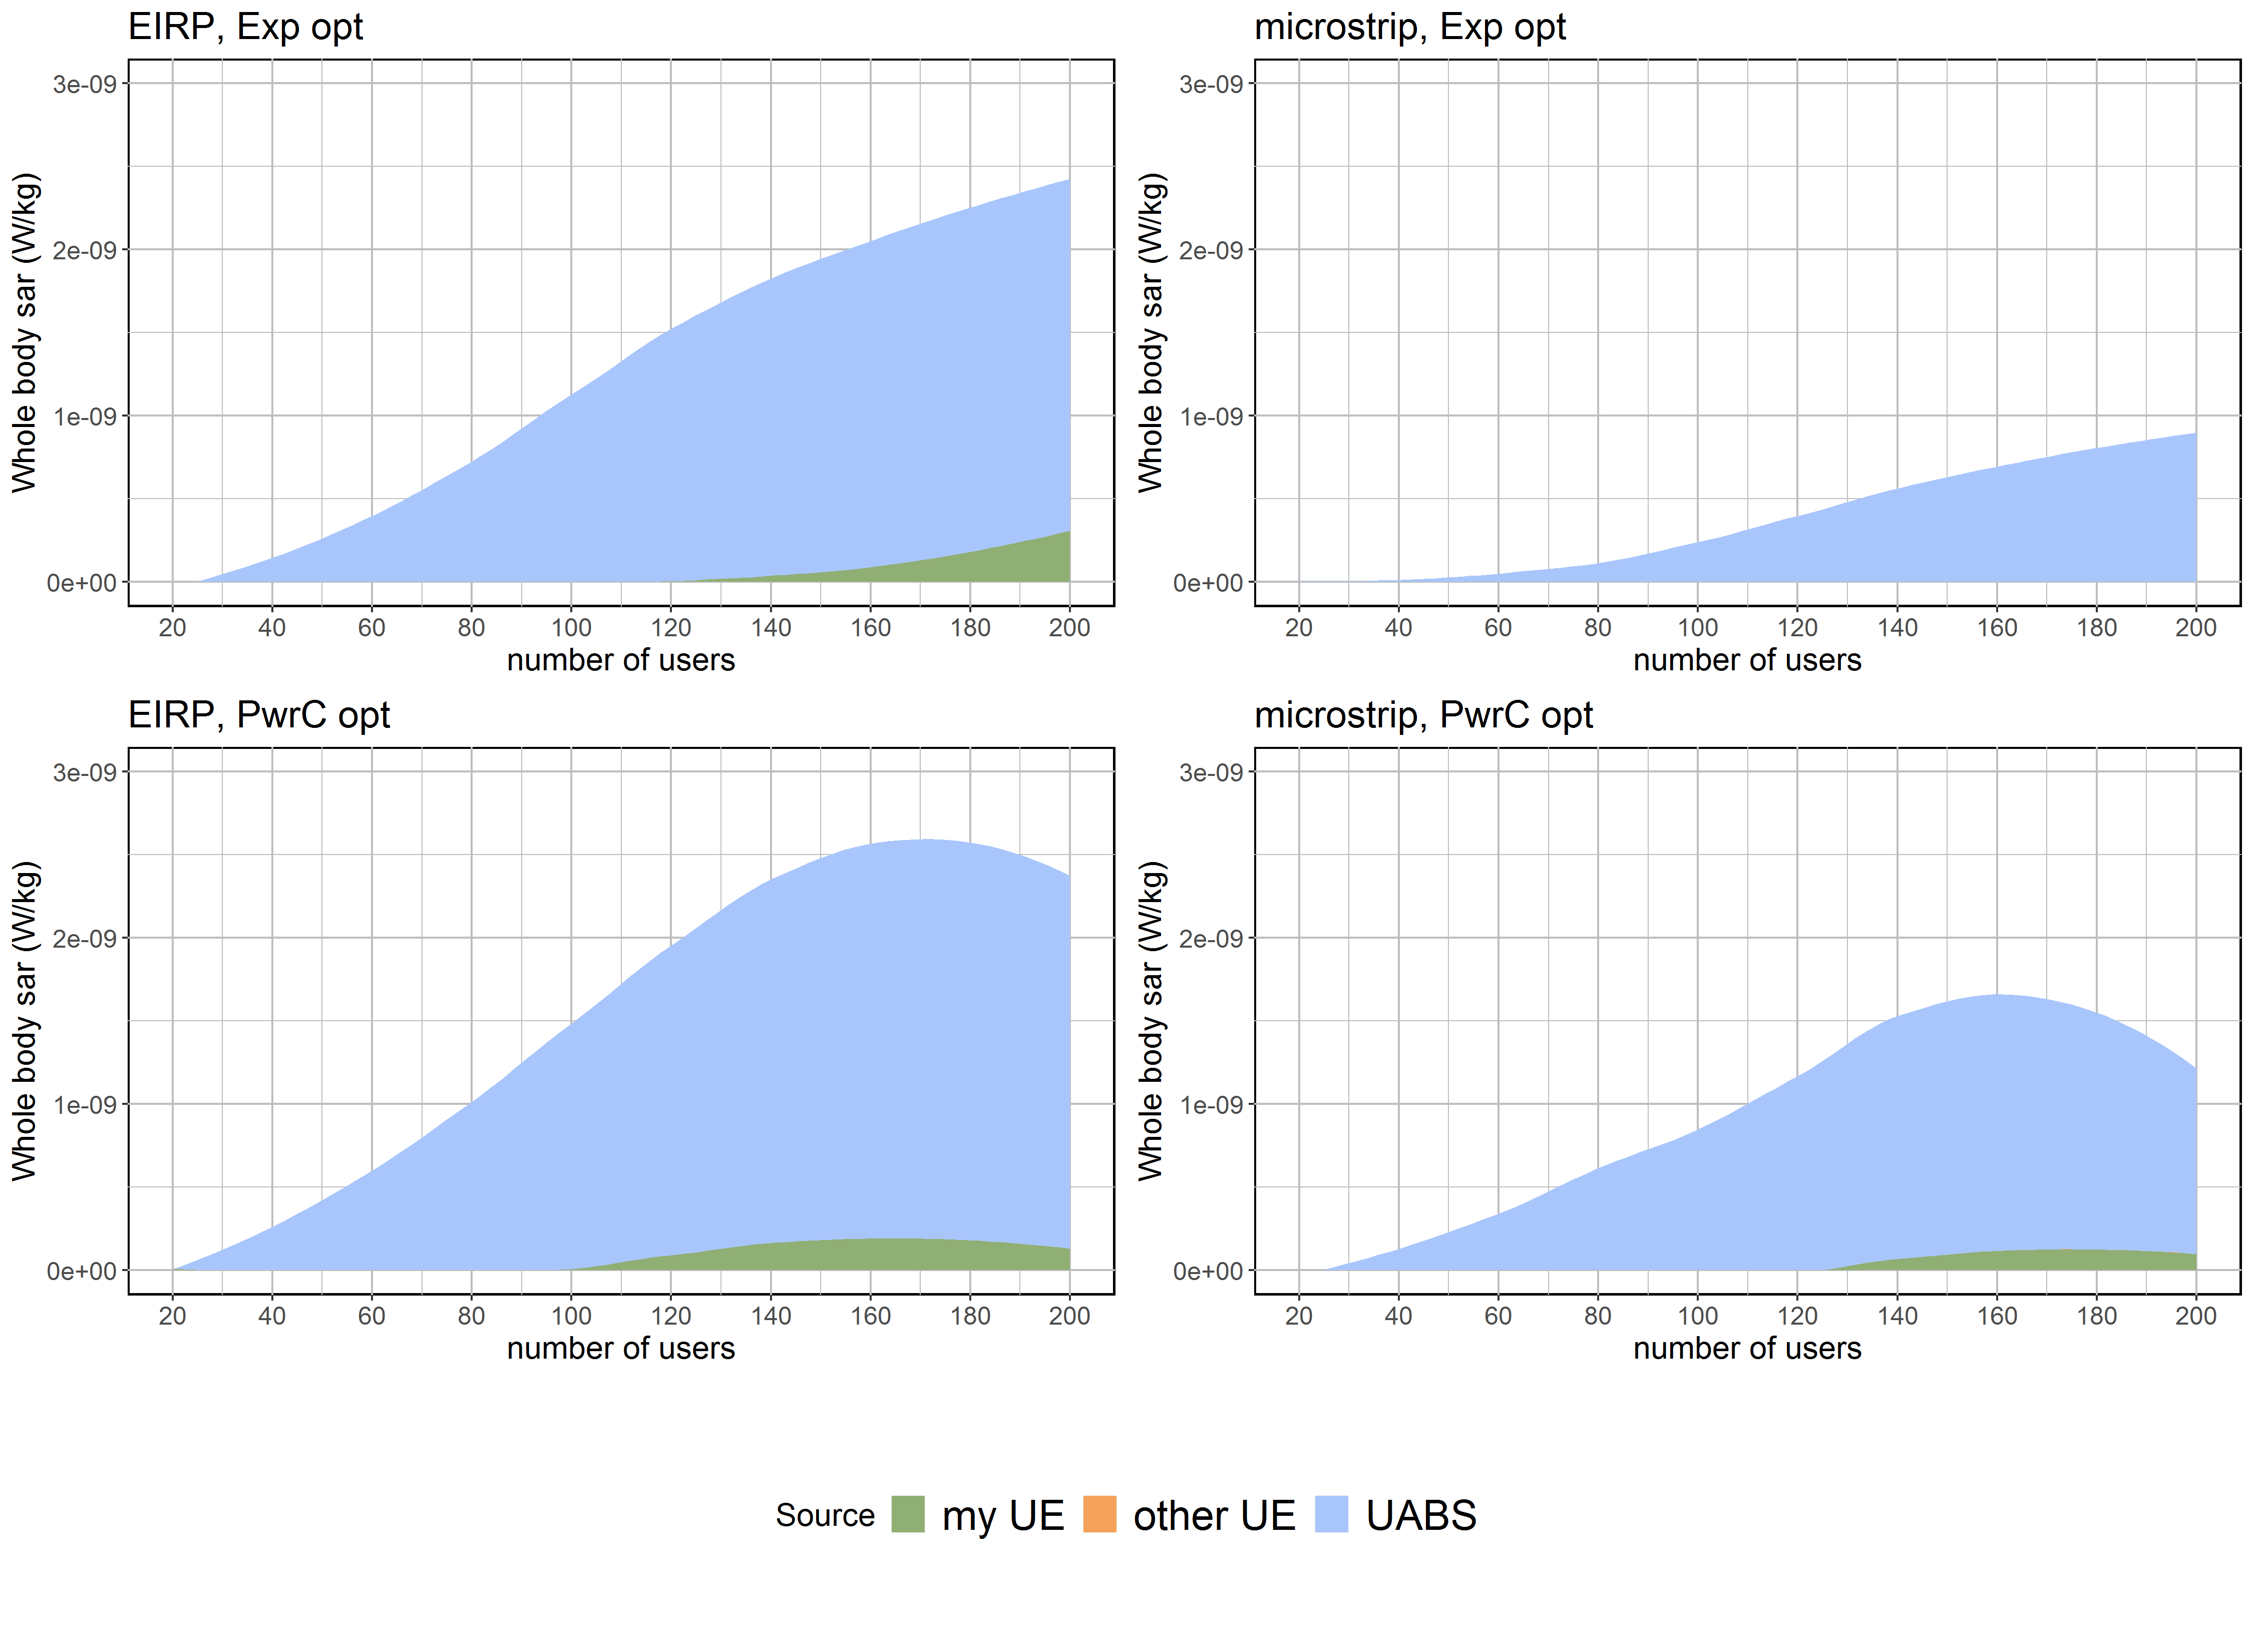
\includegraphics[width=\textwidth]{../results/s2/fhFourSources.png}
  \caption{Each figure corresponds with a certain configuration and shows how the \gls{SAR} from different sources are influenced by an increasing flying height.}
  \label{fig:s2shfourSourcesMatrix}
\end{figure}

%%%%%%%%%%%%%%%%%%%%%%%%%%%%%%%%%%%%%%%%%%%%%%%%%%%%%%%%%%%%%%%%%%%%%%%%%%%%%%%%%%%%%%%%%%%%%%%%%%%%%%%%
\FloatBarrier
\subsection{Influence of the Number of Users}
\label{s2b}

The number of covered users increases linearly compared to the number of users present in the network as shown in figure 
\ref{fig:s2uvsnumcovusers} on the right. It illustrates how an \gls{isotropicradiator} is able to reach more users 
compared to a microstrip patch antenna. Also, power consumption optimized networks are able to reach more users compared to exposure optimized networks.
This is because power consumption optimized networks will result in few high powered base stations while an 
exposure optimized network results in a lot of low powered base stations. This behaviour will further be explained in section \ref{s3}

\begin{figure}[h!]
  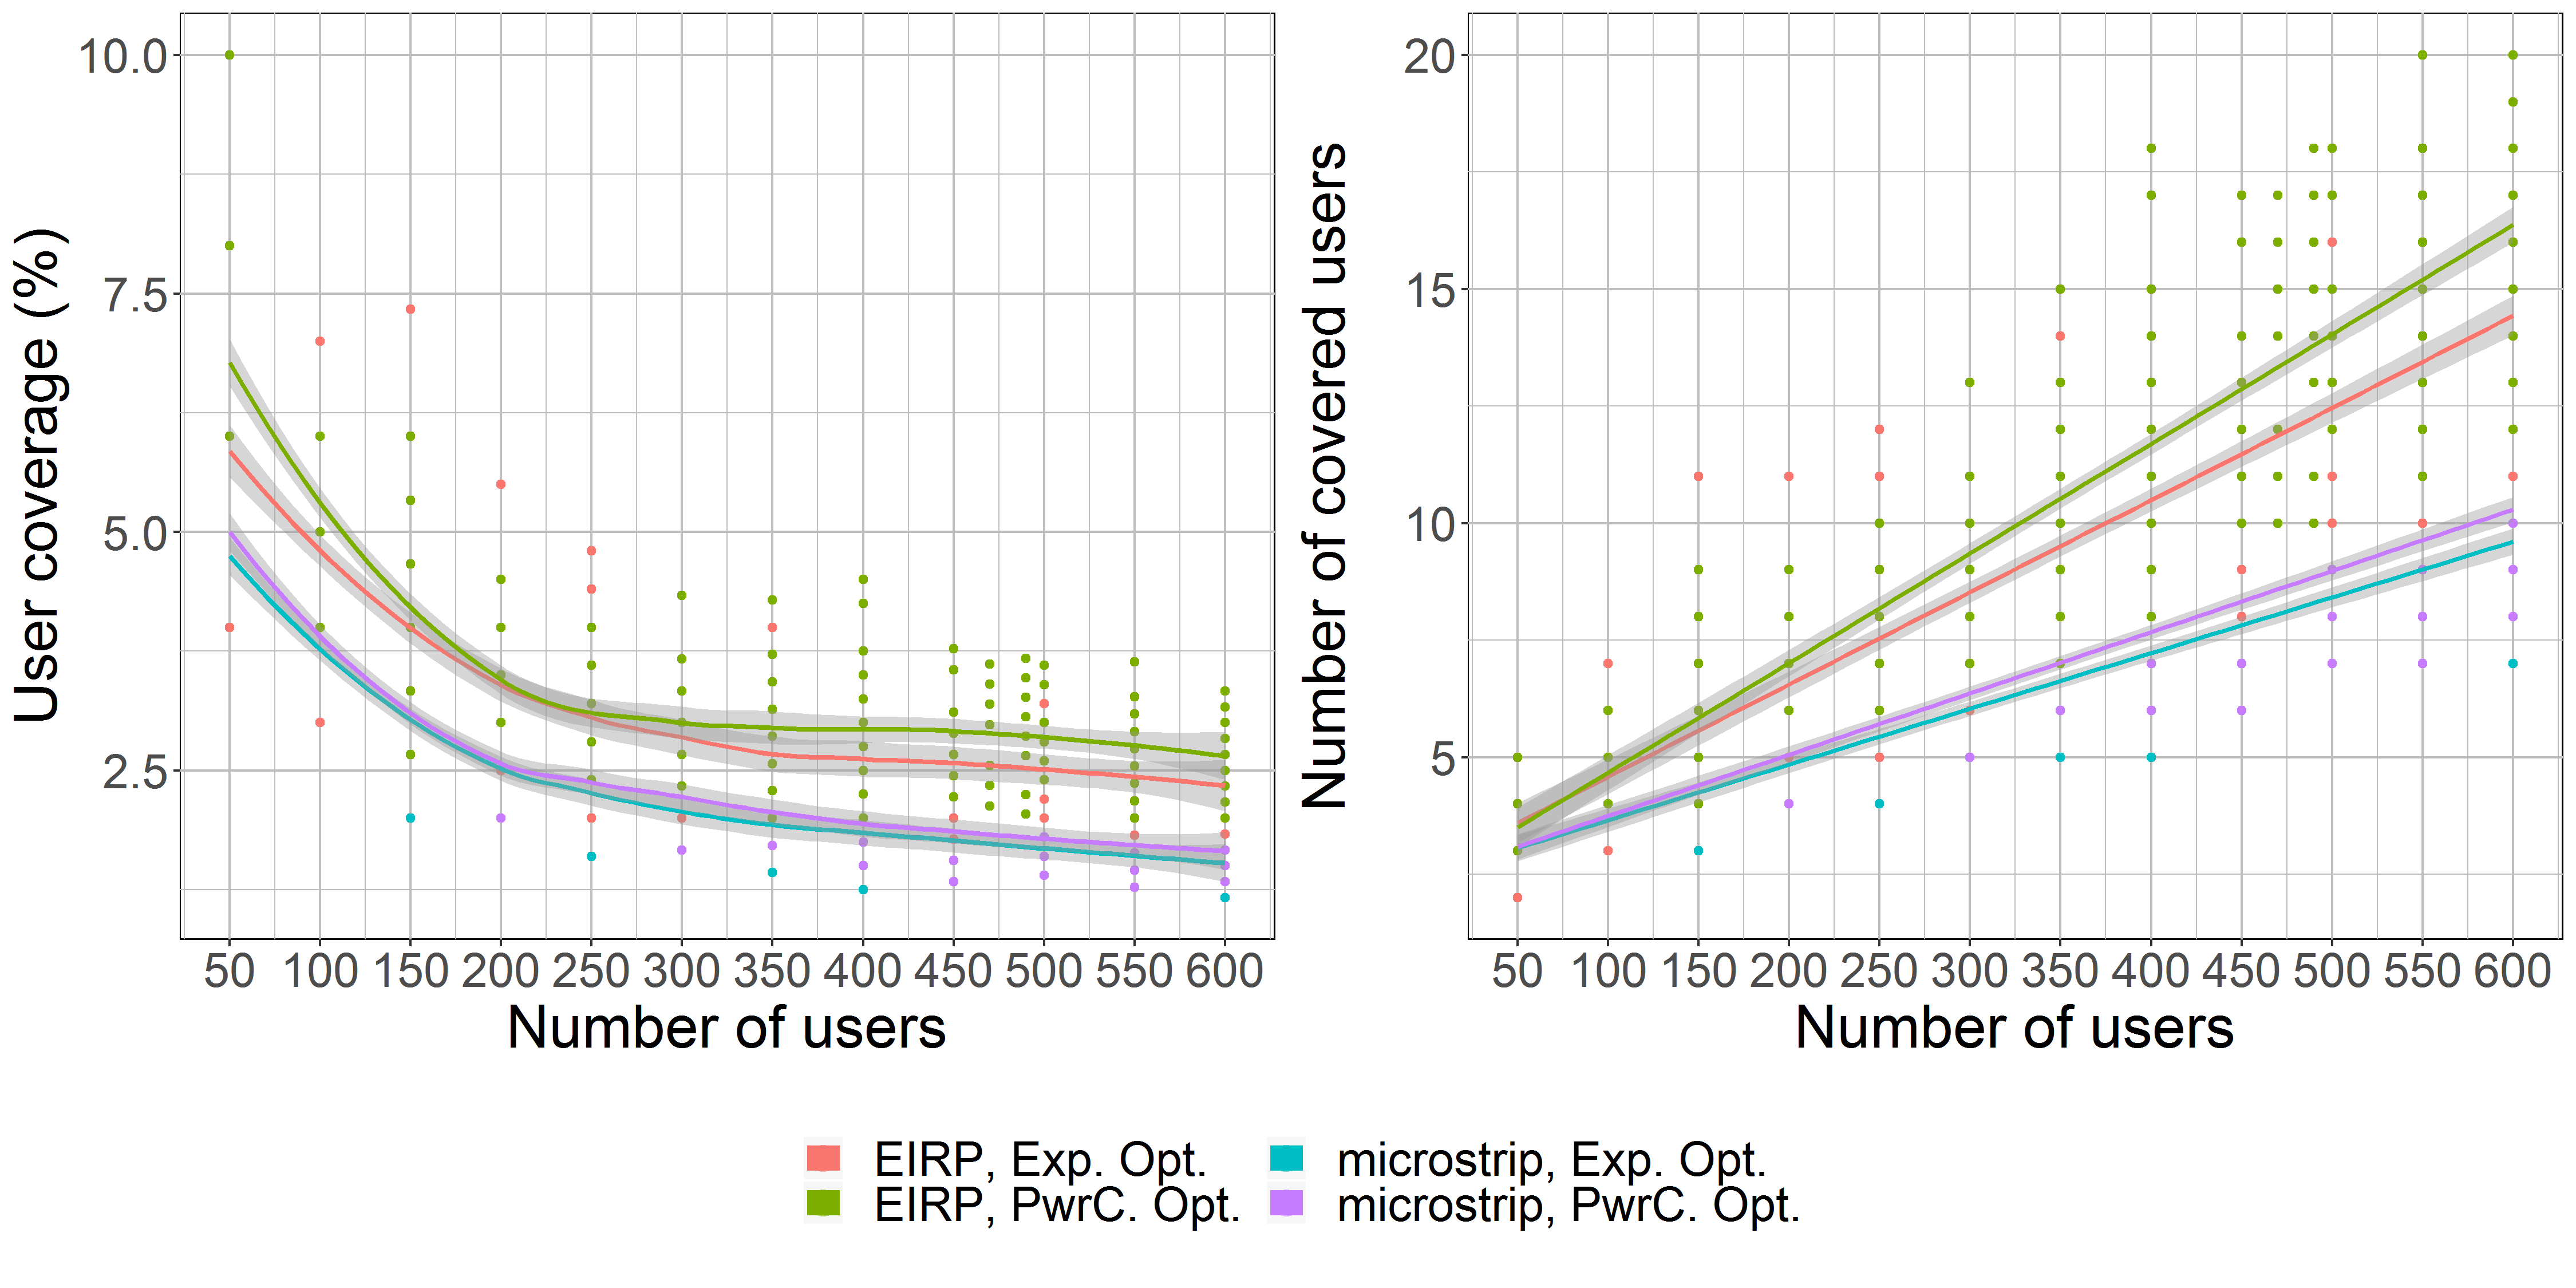
\includegraphics[width=\textwidth]{../results/s2/uvsnumdronesAndCov.png}
  \caption{The influence of increasing traffic on the user coverage.}
  \label{fig:s2uvsnumcovusers}
\end{figure}

The linear regression lines from \ref{fig:s2uvsnumcovusers} can be predicted with the equations in \ref{eq:numcovusers}.

\begin{equation}
\text{number of users =}
    \begin{cases}
      y = 0,0233x + 2,3553 & \text{if EIRP and pc}\\
      y = 0,0197x + 2,6144  & \text{if EIRP and exp}\\
      y = 0,0131x + 2,4371  & \text{if micro and pc}\\
      y = 0,0119x + 2,4652  & \text{if micro and exp}
    \end{cases} 
    \label{eq:numcovusers}      
\end{equation}

Figure \ref{fig:s2uvsnumcovusers} on the left shows the percentage of covered users that follow out of \ref{fig:s2uvsnumcovusers} on the right by taking the equations 
from \ref{eq:numcovusers} and dividing them by $x$.
This results in a decreasing logarithmic behaviour because the regression lines from  \ref{fig:s2uvsnumcovusers} have a slope of less than 0.5.
This means that the percentage of covered users for a sparsely populated network is more compared to the percentage of users in high dense populations.

\begin{figure}[h!]
  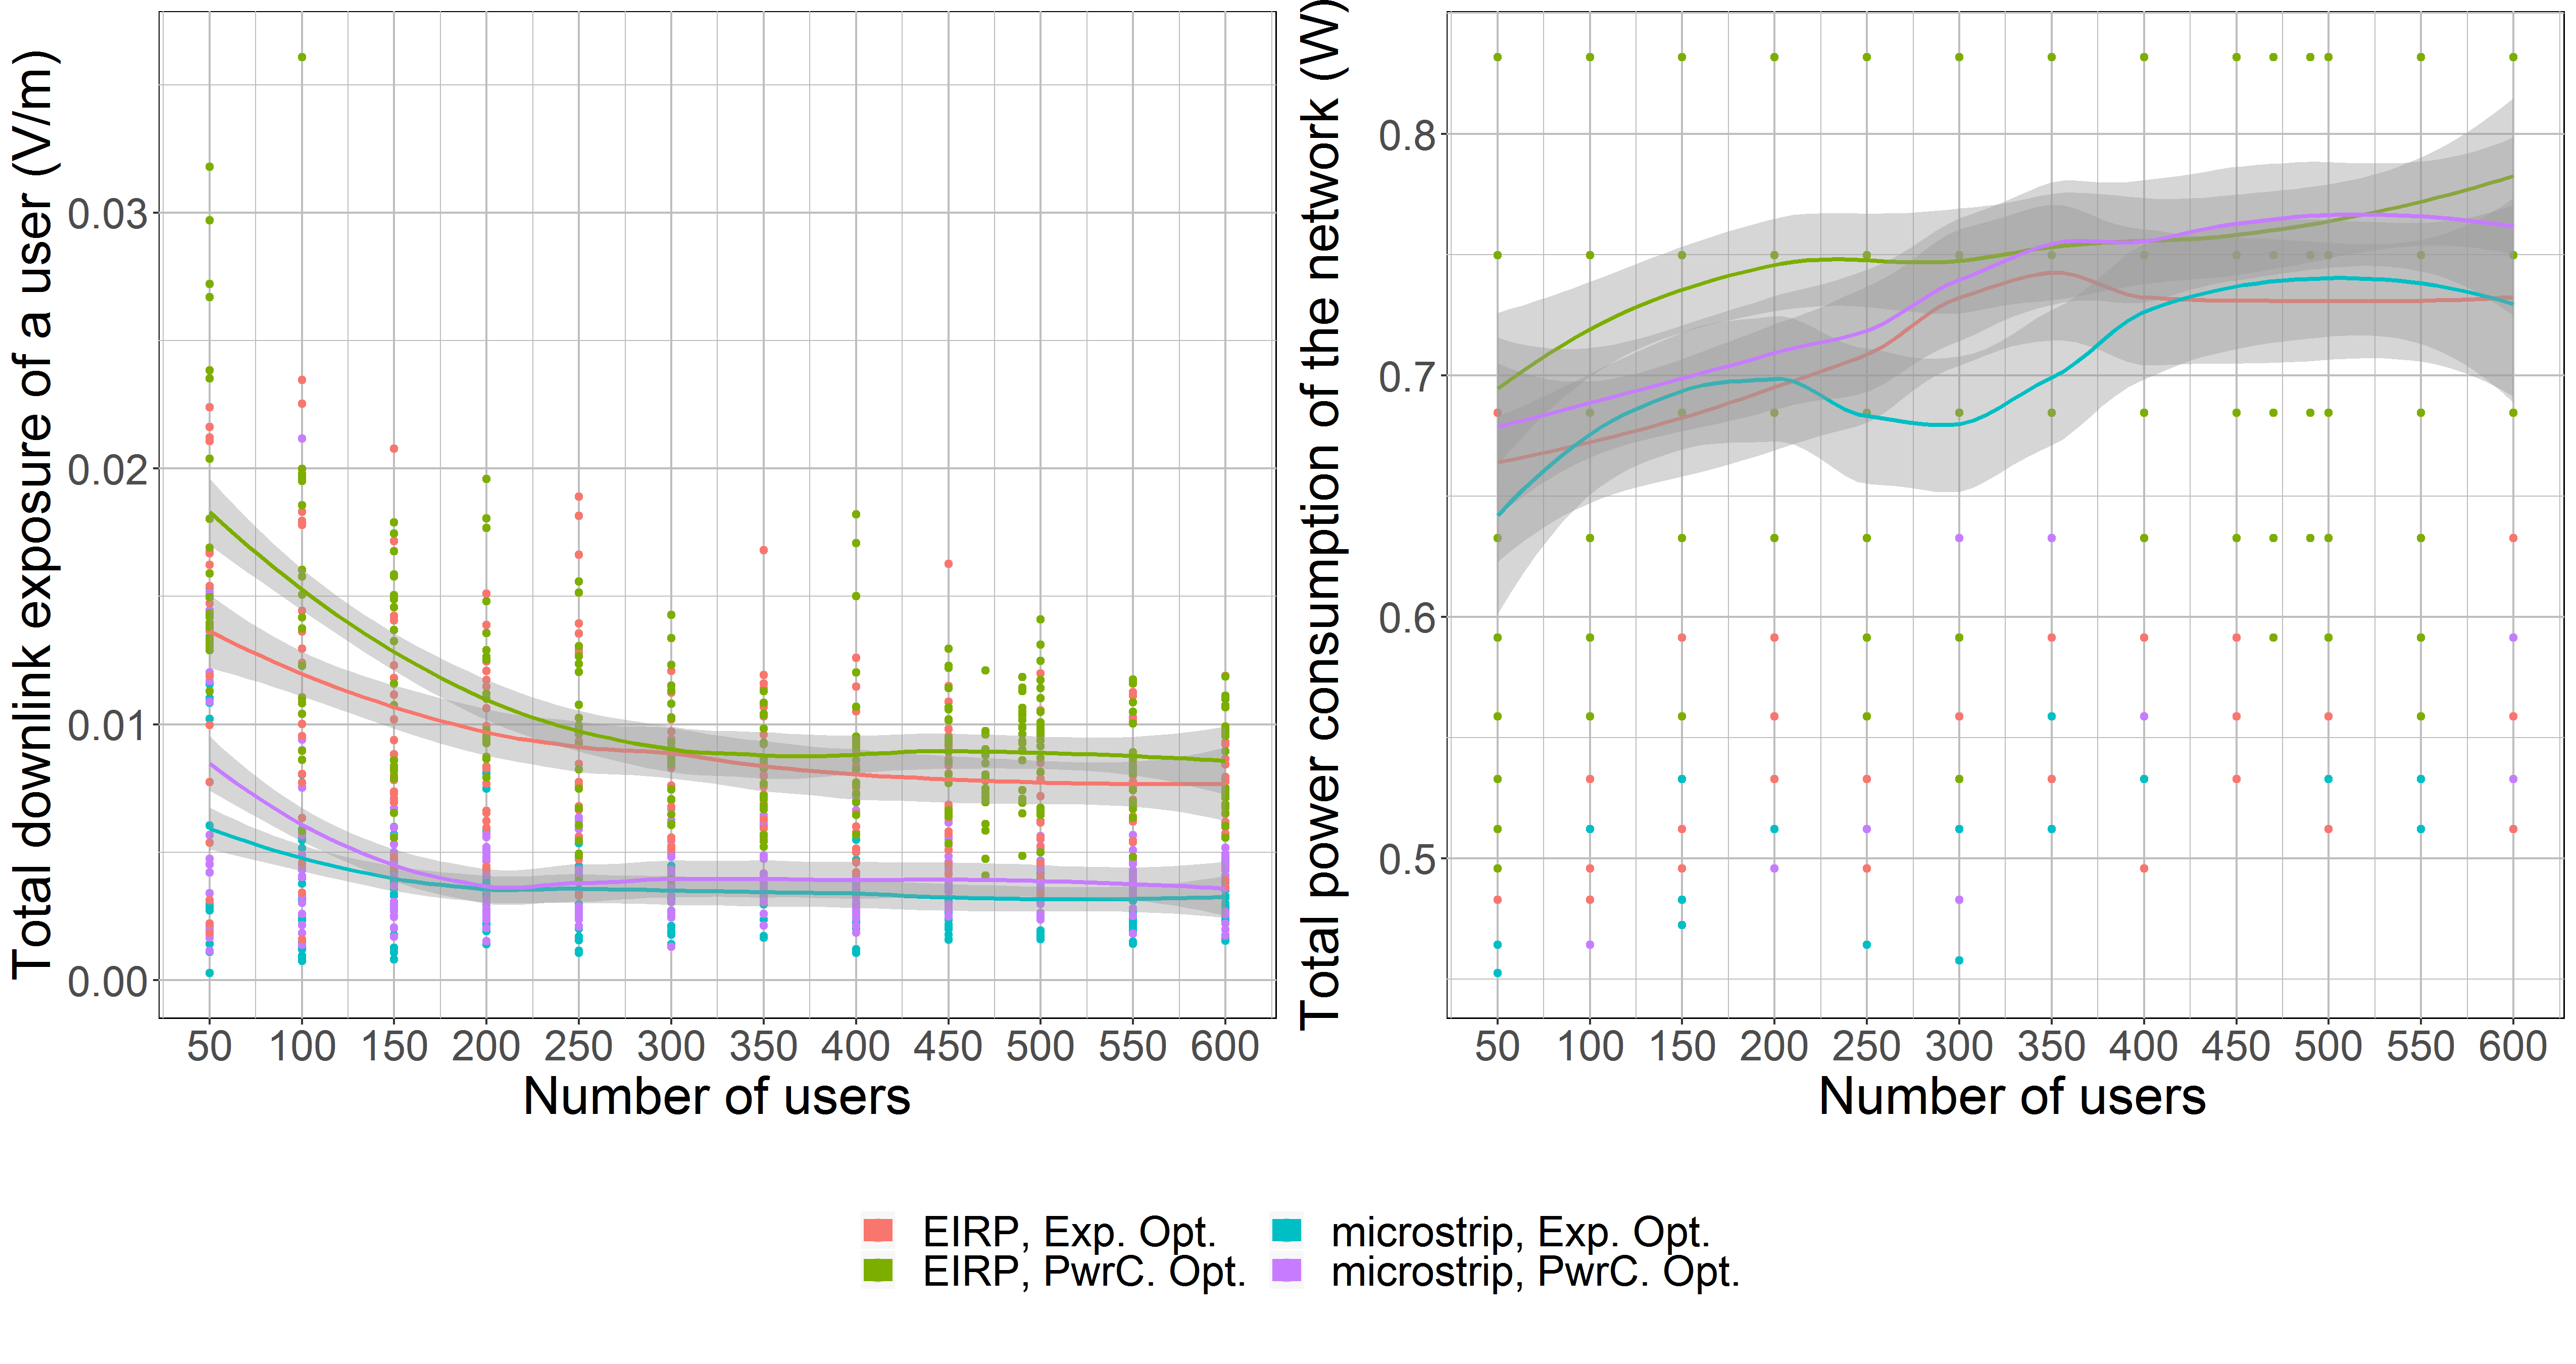
\includegraphics[width=\textwidth]{../results/s2/uvsdlAndPc.png}
  \caption{These two figures show how various sizes of population influence the downlink electromagnetic radiation of the average user (left) and 
  power consumption of the entire network (rights) for one \gls{UABS} available in the network.}
  \label{fig:s2b_dlAndPc}
\end{figure}

The downlink exposure is shown in figure \ref{fig:s2b_dlAndPc} on the left and is directly influenced by the percentage of covered users. 
The average electromagnetic exposure decreases when more users become uncovered. Since an \gls{isotropicradiator} in a power consumption optimized network (green)
will have the highest coverage, also the \gls{DL} electromagnetic radiation from \gls{UABS}s will be higher compared to other configurations.
Despite the fact that the percentage of covered users decreases, the effective number of covered users increases. The power consumption of the only 
active \gls{UABS} slightly increases in order to serve those covered users.


Figure \ref{fig:s2fourSourcesMatrix} investigates the assets of each source contributing to the total \gls{SAR}. All four 
configurations show that base stations are the main source of electromagnetic radiation.
Figure \ref{fig:s2uvsnumcovusers} already 
showed that for sparsely populated networks, a higher percentage is covered so the weighted average of the \gls{UL} \gls{SAR} will also be higher. 
When the population becomes more dense,
more users become uncovered which decreases the weighted average of the \gls{UL} \gls{SAR}.
The chart also proves once again that the far-field radiation from \gls{UE} can be neglected. The \gls{SAR} from 
neighbouring devices is not zero as it looks from figure \ref{fig:s2fourSourcesMatrix} but is just really low compared to the much higher
\gls{SAR}-values from other sources.

\begin{figure}[h!]
\centering
  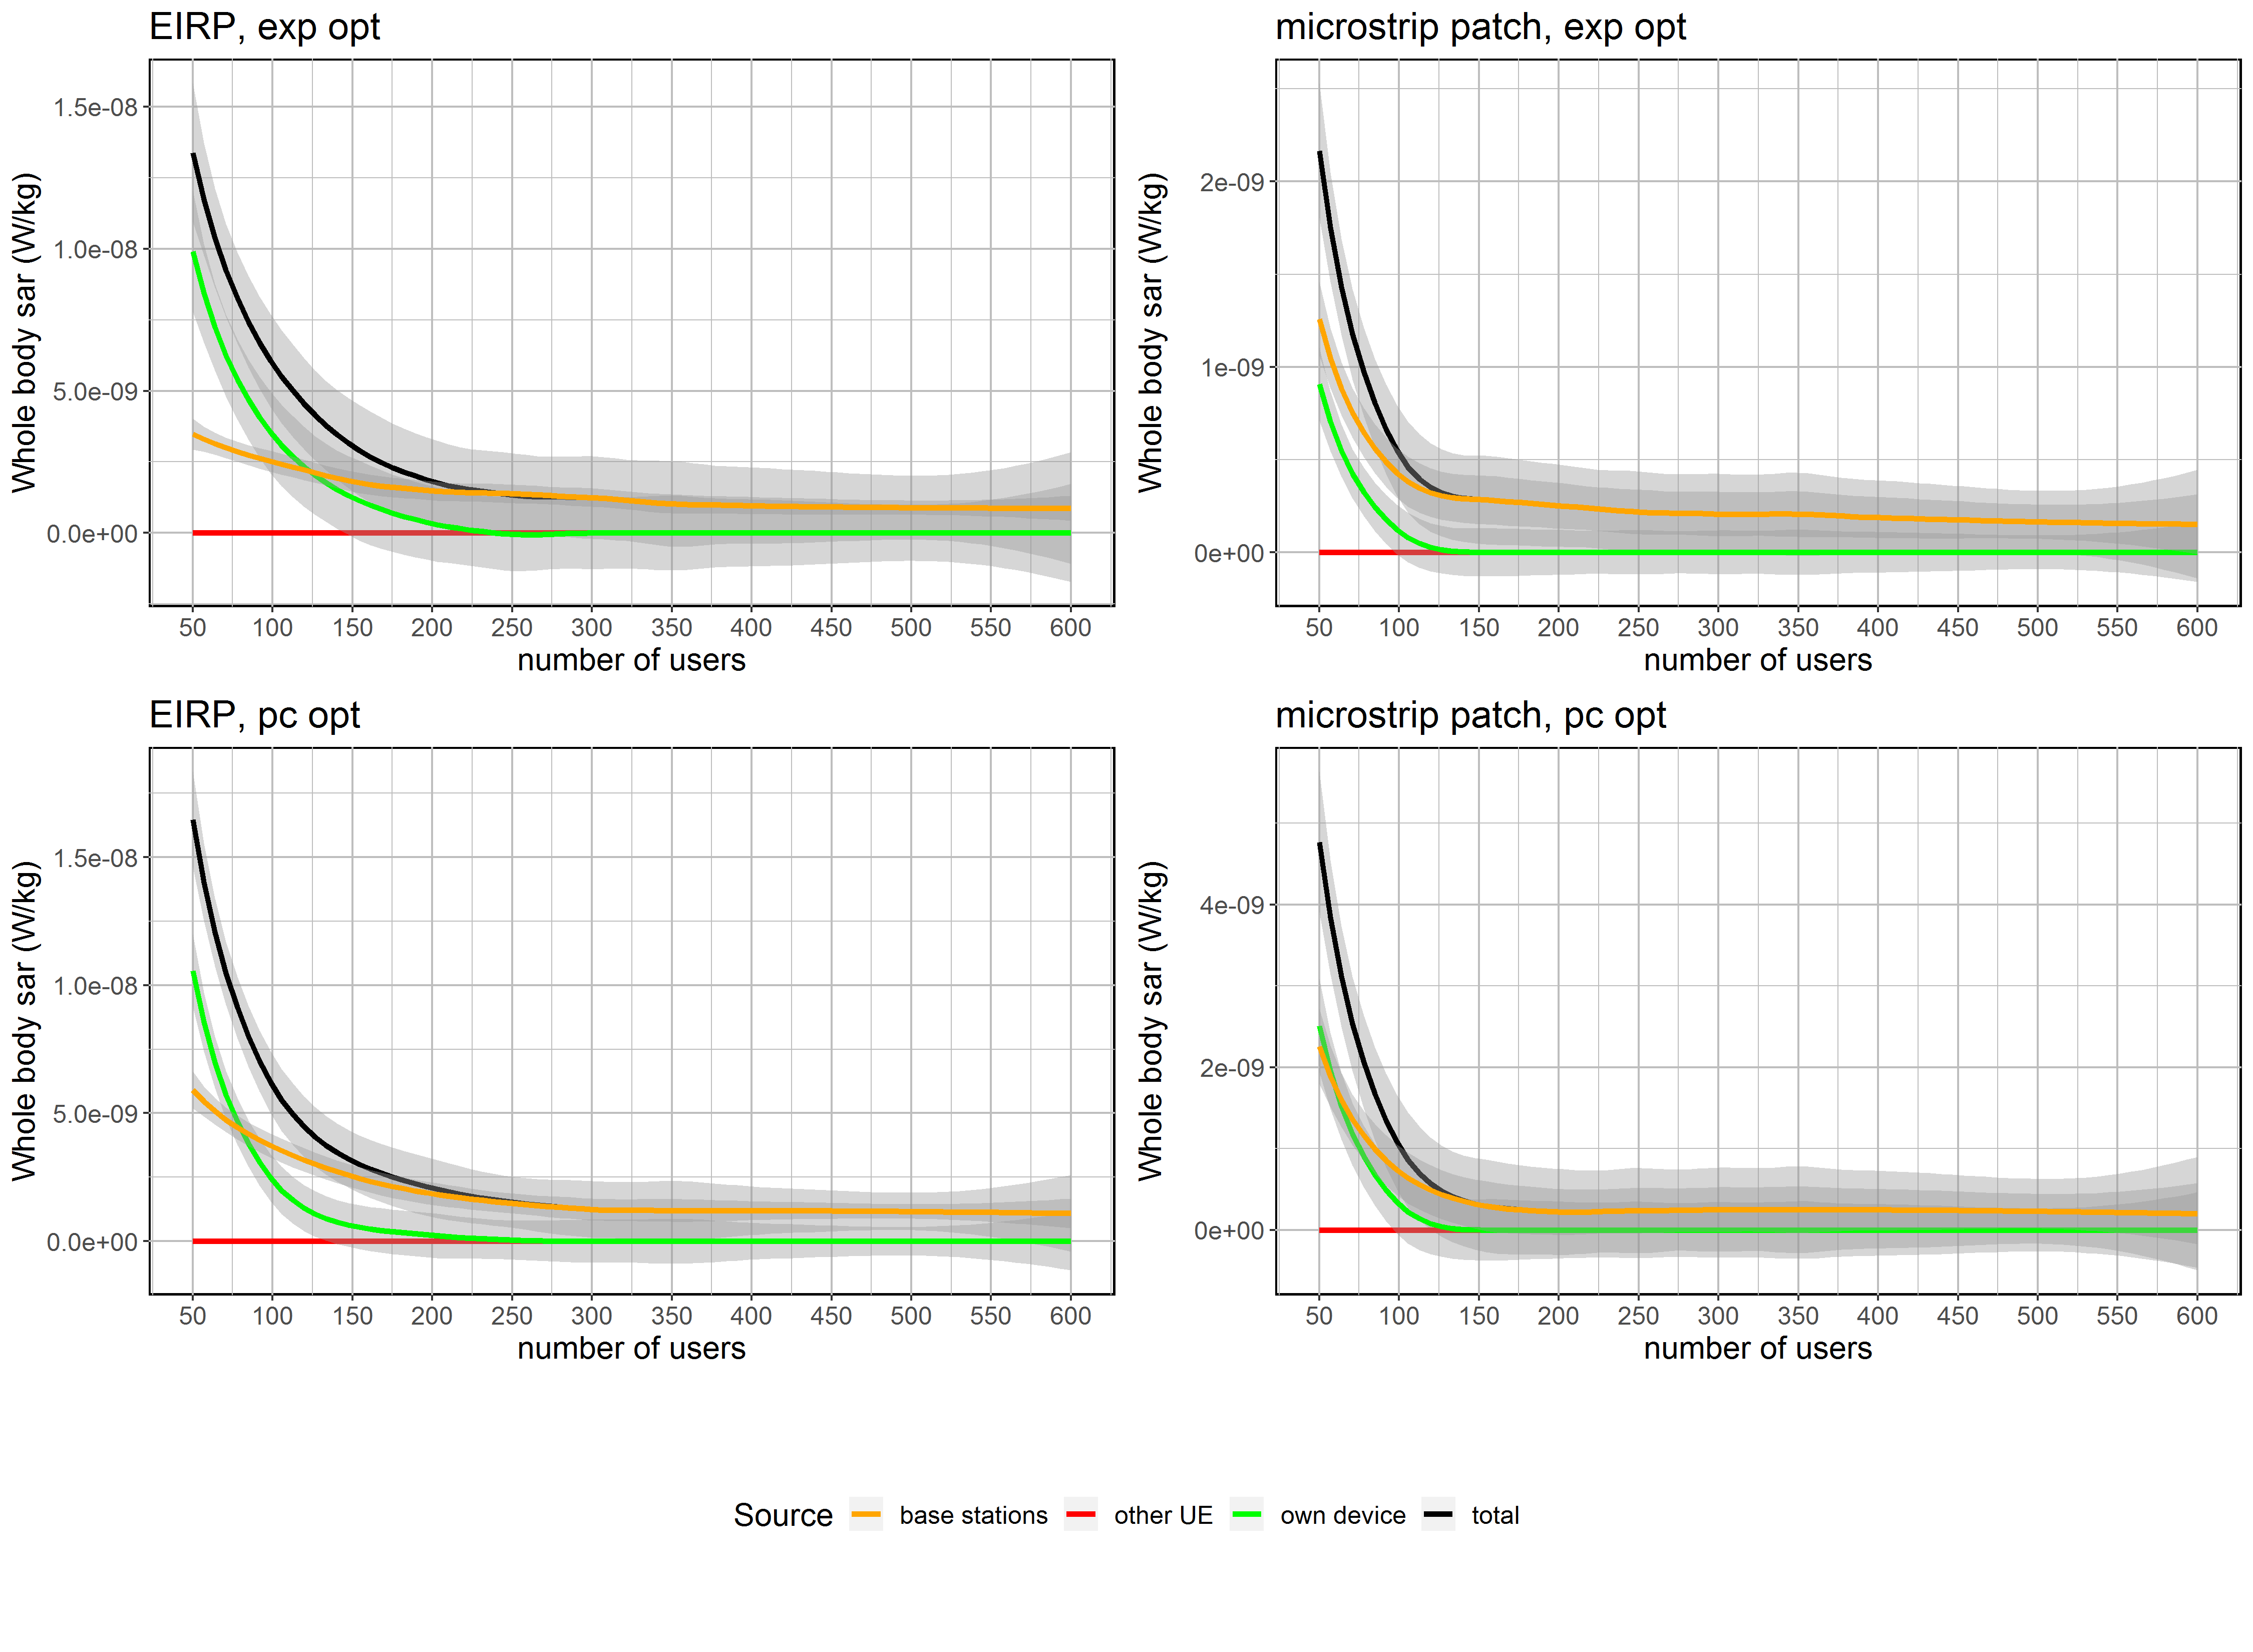
\includegraphics[width=\textwidth/6*5]{../results/s2/uFourSources.png}
  \caption{This figure shows how different sources are influenced by an increasing number of users. }
  \label{fig:s2fourSourcesMatrix}
\end{figure}

While the population grows, more and more users become uncovered causing the average SAR to drop. 
However, this does not conclude that  by increasing the population, the SAR of a user who is directly beneath a \gls{UABS} would be less.
To investigate this, a user is positioned in the middle of the city centre of Ghent and a \gls{UAV} is positioned above him. Initially, only 
49 people are active around him. The \gls{SAR} of our central user is monitored while the population around him is growing.
Figure \ref{fig:connectionMap} shows with the black lines which users are connected. The left map is for only 50 users and 
shows that only one user is connected besides our central user. The map on the right is taken with 600 users and shows much more connected users.

\begin{figure}[h!]
\centering
  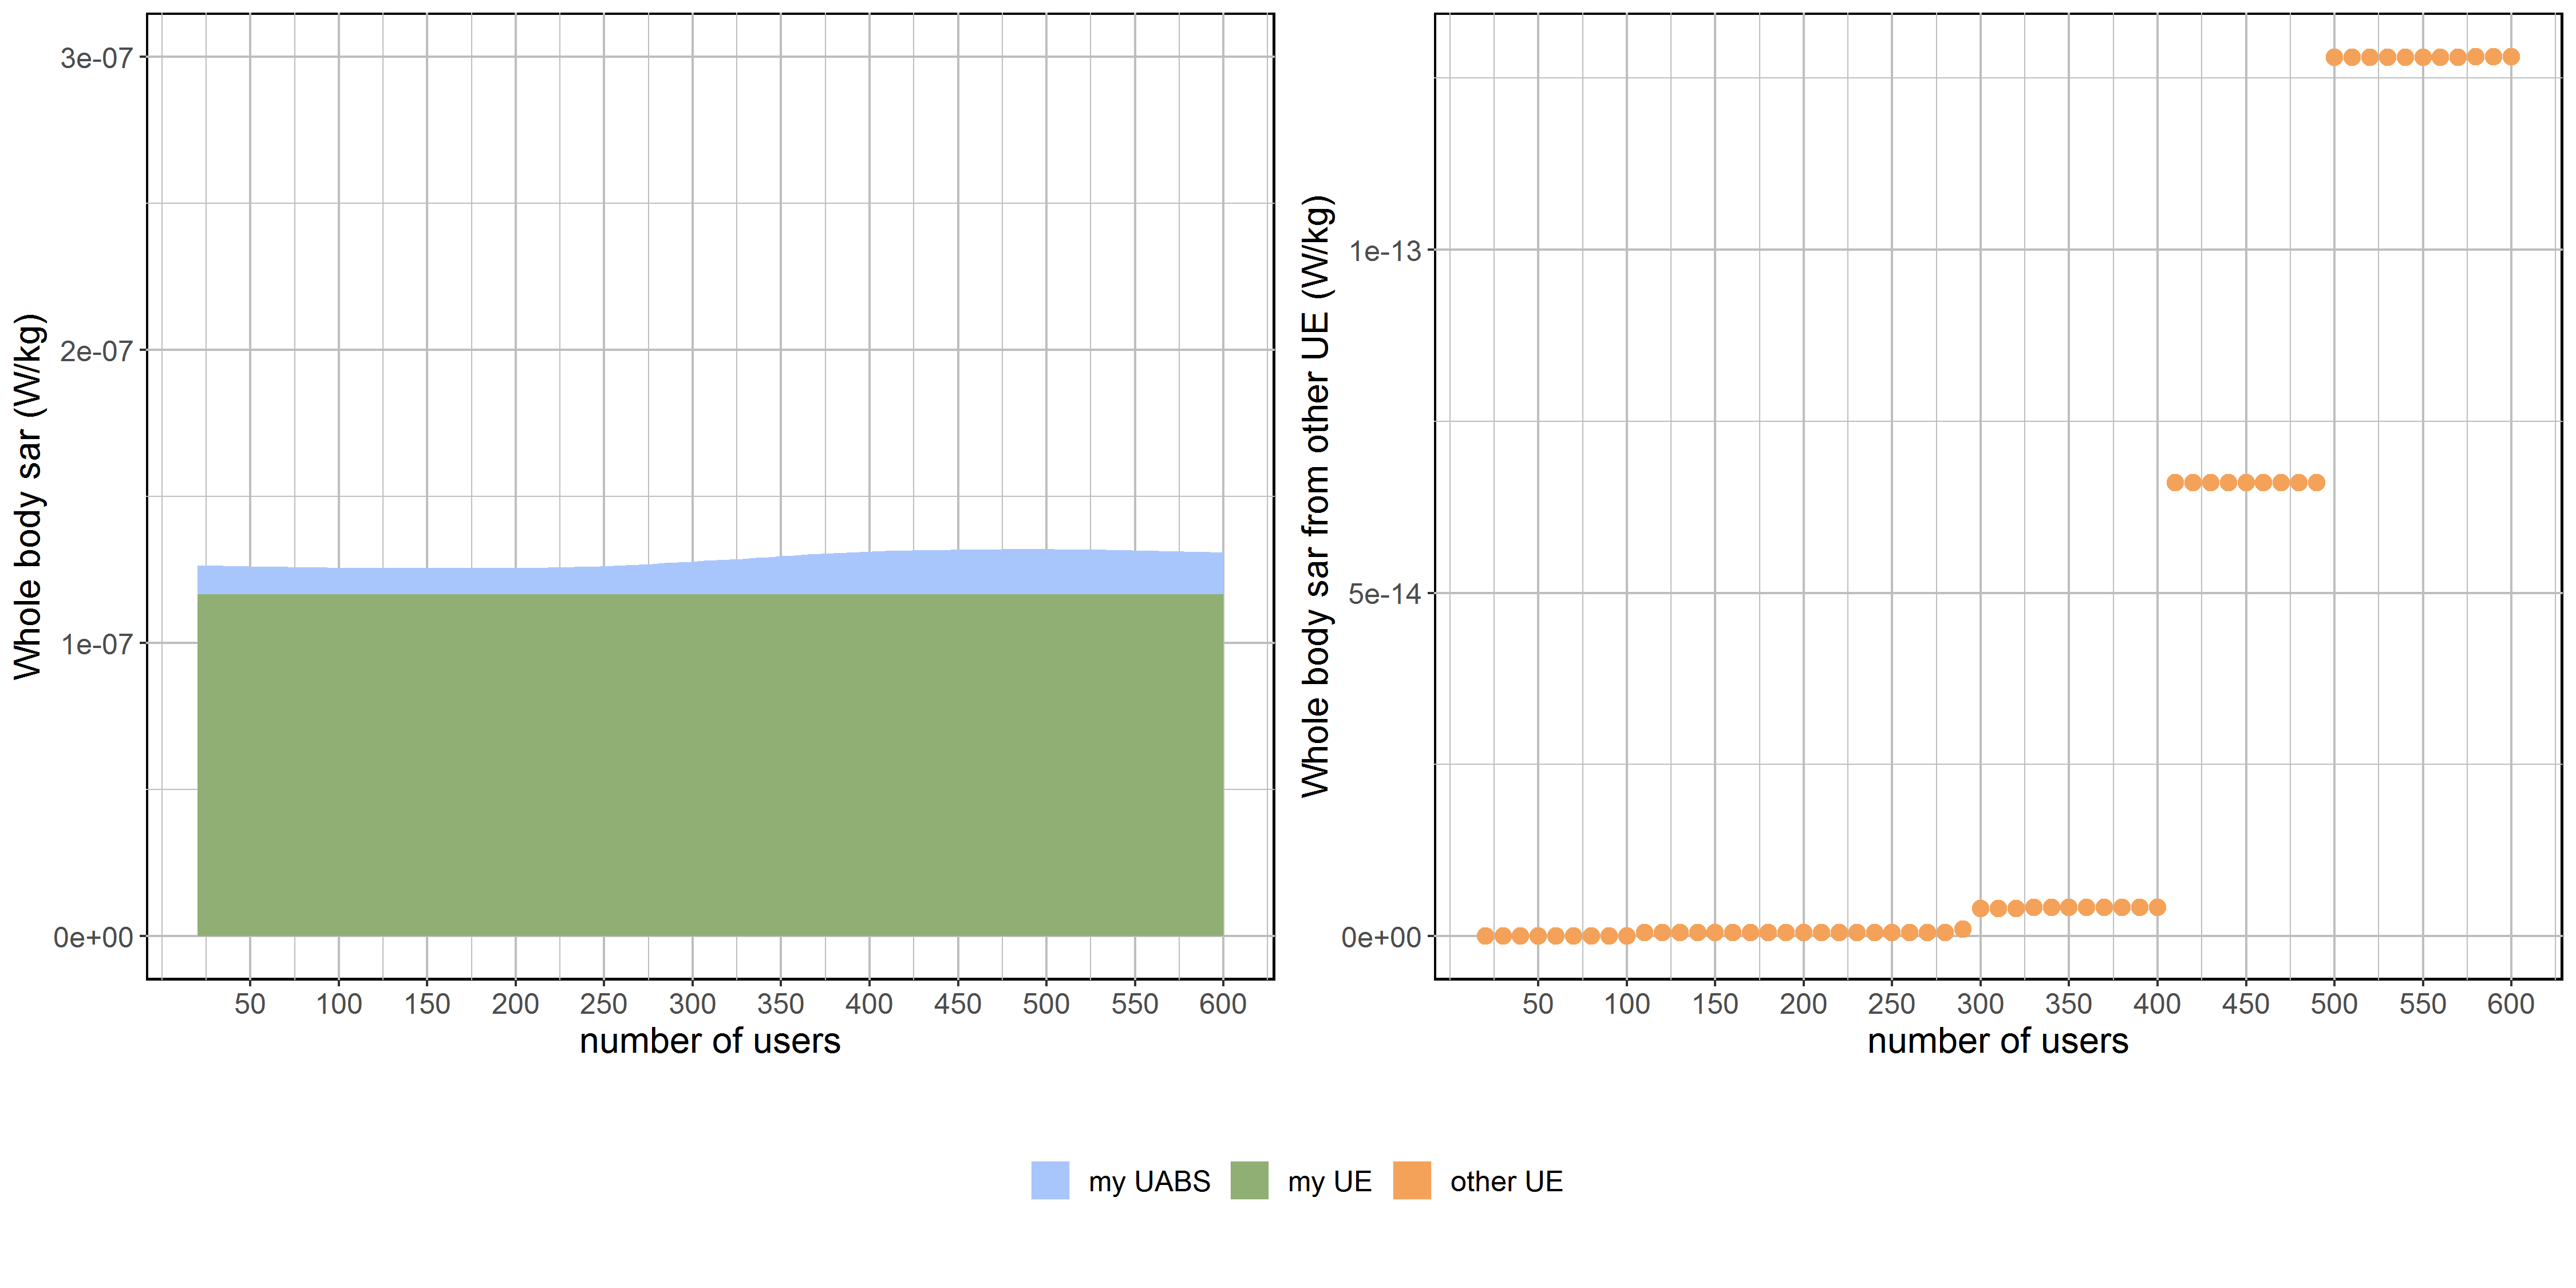
\includegraphics[width=\textwidth/6*5]{../results/s2/uvsulsarcentralUser.png}
  \caption{SAR-values for the user who is directly beneath the only \gls{UABS} available.}
  \label{fig:uvsulsarcentralUsers}
\end{figure}

Scenario 1 already showed that the \gls{SAR} from the user's own device is only influenced by the flying height. 
The flying height for this experiment is fixed and the \gls{UL} \gls{SAR} from his device should therefore be also a constant. 
A hypothesis that is confirmed by figure \ref{fig:uvsulsarcentralUsers}.
The \gls{SAR} from the \gls{UABS} experiences a slight increase. When the population grows, more users become available 
and some will spawn near the central user. The \gls{UABS} will likely decide to cover these users as well as visible in figure \ref{fig:connectionMap}.
These users might have a slightly 
worse path loss because of obstructing buildings or somewhat bigger distance. The \gls{UABS} reacts to this by increasing 
his power consumption causing an increase in the \gls{DL} \gls{SAR} for the central user.

The far-field radiation from \gls{UE} is very low as mentioned before and is therefore not visible in figure \ref{fig:connectionMap} 
on the left. It is therefore illustrated in a separate chart on the right. 
It shows that the \gls{SAR}  from other \gls{UE} indeed increases. This is normal 
behaviour considering that more and more people become available around the central user of which some will be connected to the \gls{UABS}
and therefore also emitting radiation.

\begin{figure}[!htb]
\minipage{0.50\textwidth}
  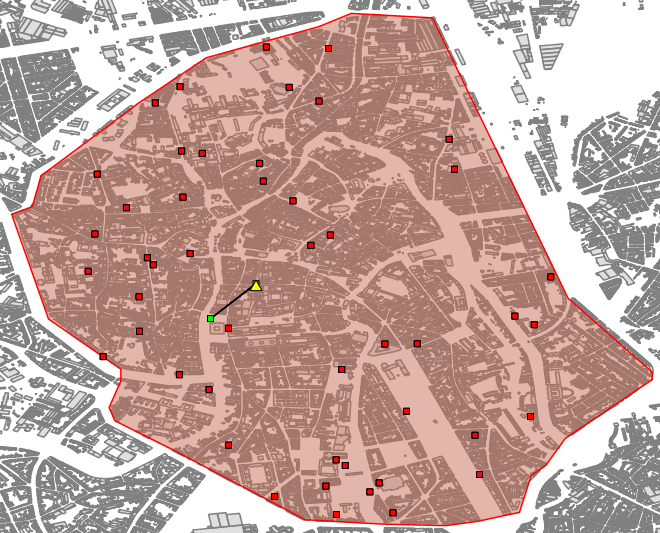
\includegraphics[width=\linewidth]{../images/connectionsMap50Users.png}
\endminipage\hfill
\minipage{0.50\textwidth}%
  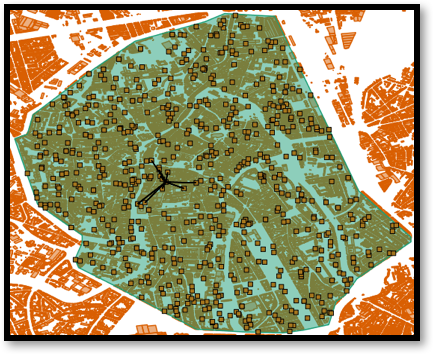
\includegraphics[width=\linewidth]{../images/connectionsMap600Users.png}
\endminipage
  \caption{Overview of which users are connected to the \gls{UABS}. The map on the left is for 50 active users while the map on the right is with 600 active users.}
  \label{fig:connectionMap}
\end{figure}
%%%%%%%%%%%%%%%%%%%%%%%%%%%%%%%%%%%%%%%%%%%%%%%%%%%%%%%%%%%%%%%%%%%%%%%%%%%%%%%%%%%%%%%%%%%%%%%%%%%%%%%%%%%%%s
\section{Scenario 3: Unlimited \gls{UAV}s}
\label{s3}

This scenario has just like the previous scenario much more users in the network 
and investigates the same cases which includes the variable flying height and the variable number of  users.
The only difference is that the restriction of only one \gls{UABS}s is dropped.

\subsection{Influence of the Flying Altitude}
\label{S3A}

The first case of this scenario examines how the network behaves for various flying heights and a fixed number of 224 users.
Scenario 2 already explained that when only one \gls{UAV} is available, a power consumption optimized network won’t result in a low 
powered network. In this scenario, there is no limitation on the number of \gls{UAV}s and the network remains thus unaltered after the decision 
algorithm is done. Figure \ref{fig:s3a_dlAndPc} clearly proves that the different optimization strategies work as intended.
Power consumption optimized networks have indeed a lower power consumption but therefore result in higher electromagnetic radiation.
On the other hand, an exposure optimized network will reduce the electromagnetic exposure by using more \gls{UAV}s and thence also increasing the network's power consumption.
This conclusion was already made  in \cite{J1} and is supported by these results.

\begin{figure}[h!]
  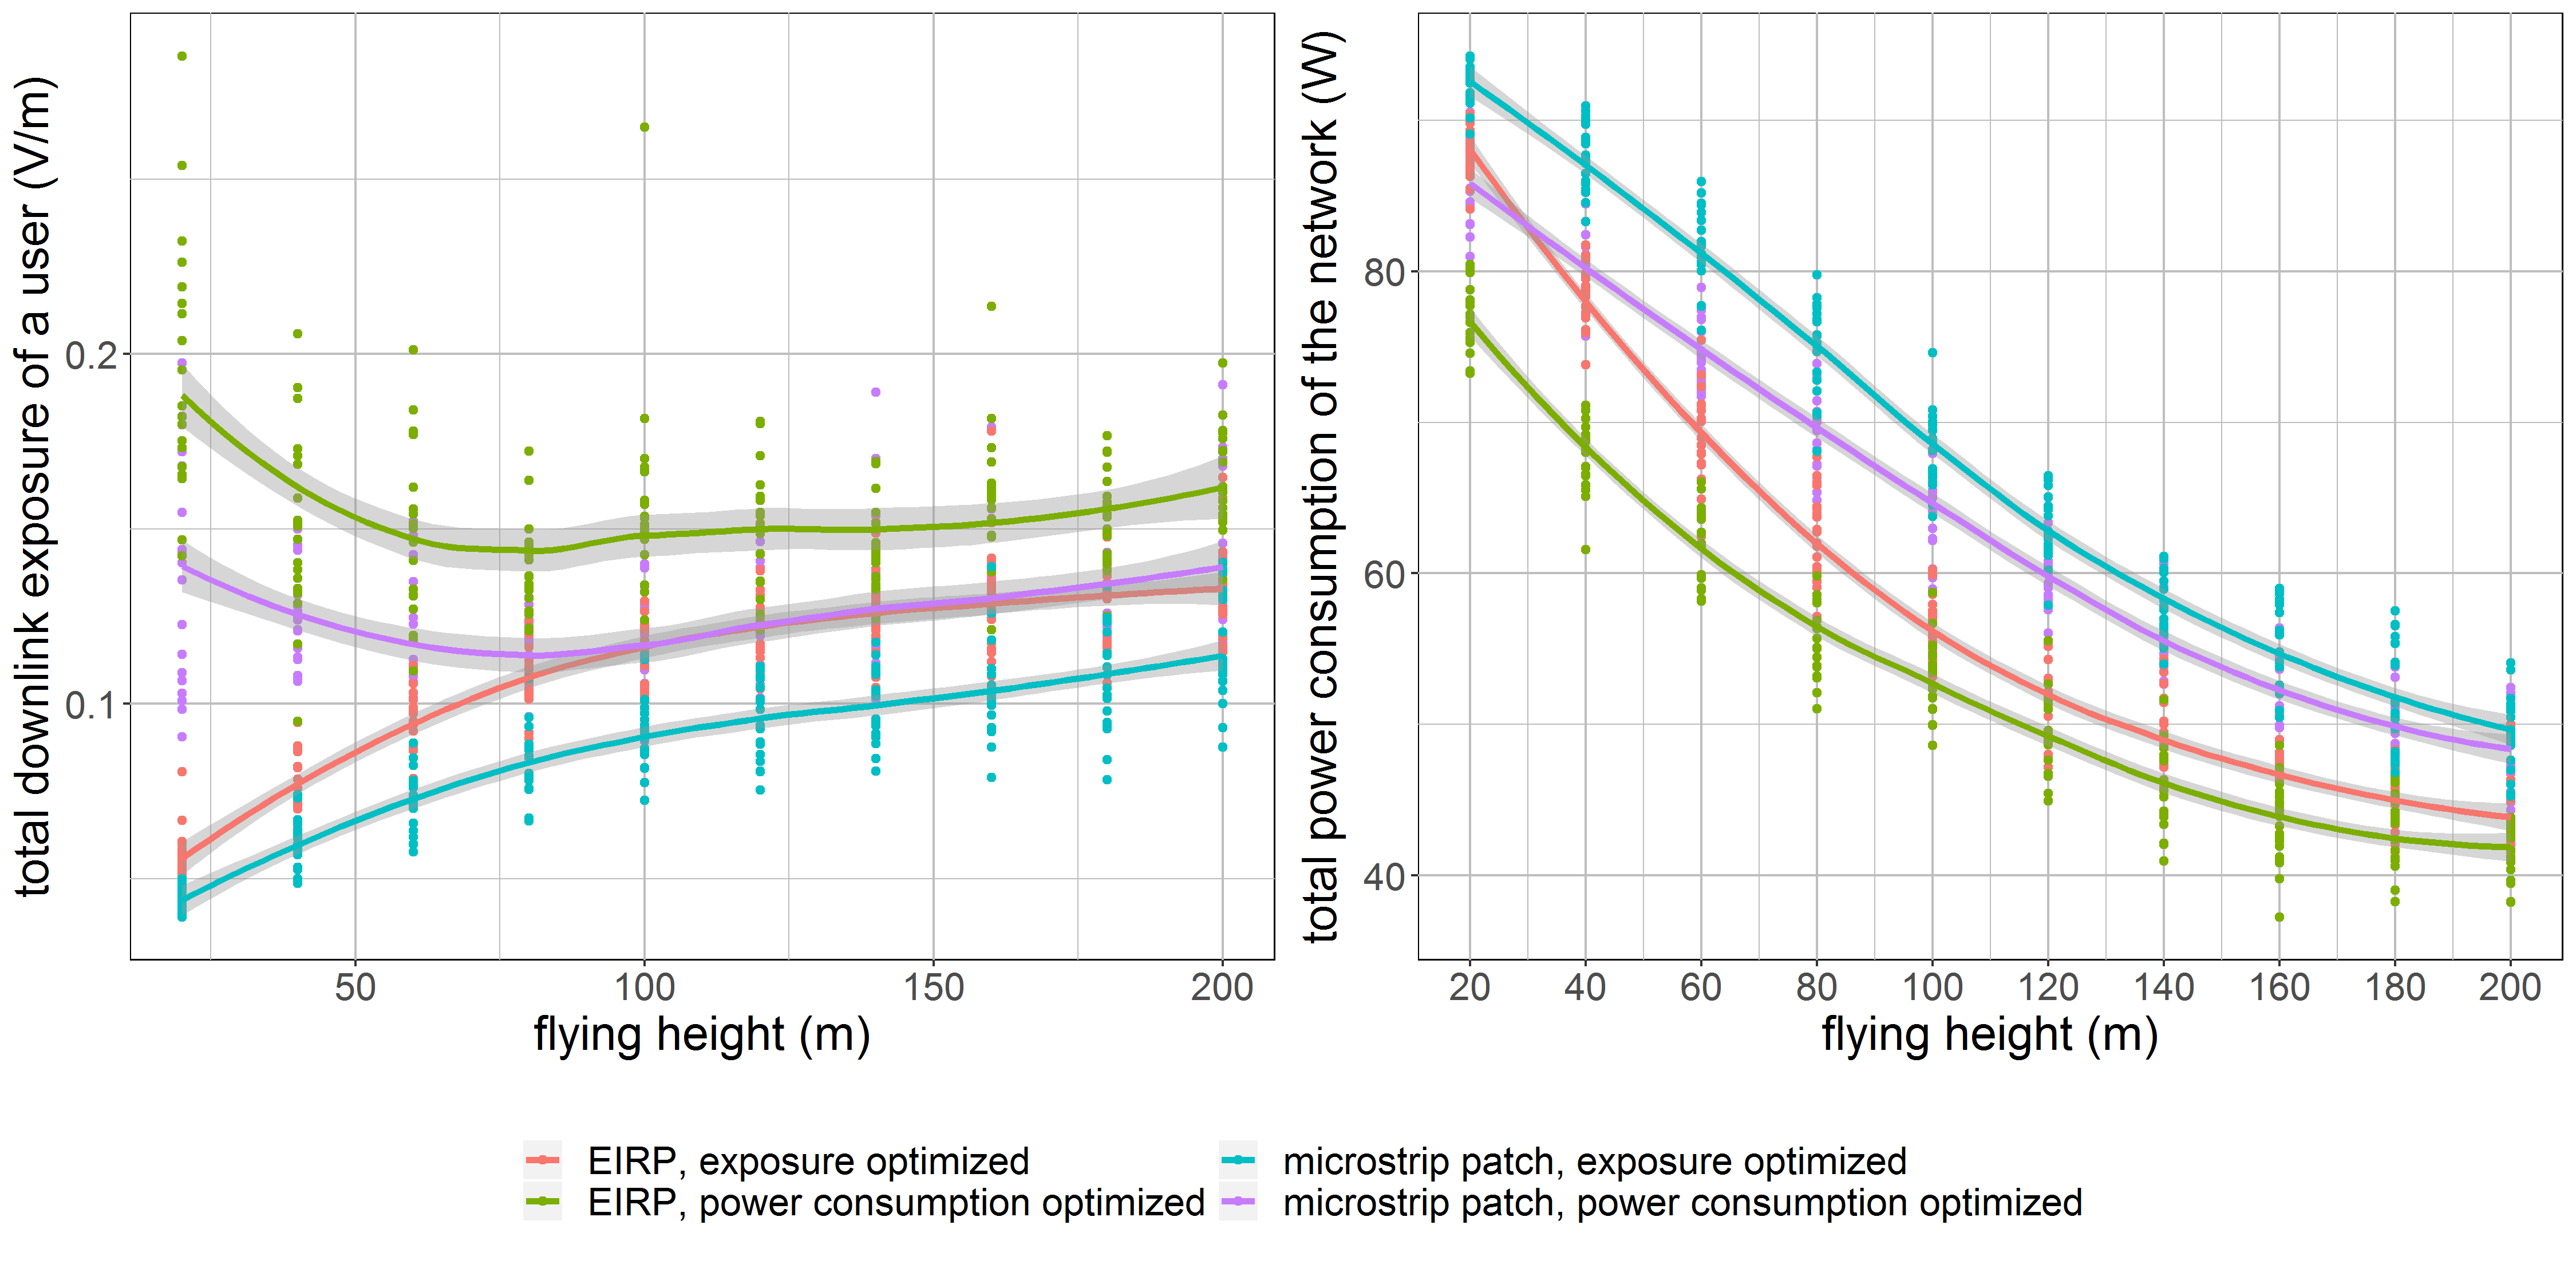
\includegraphics[width=\textwidth]{../results/s3/fhvsdlAndPc.png}
  \caption{
    These two figures show how the flying height influences the downlink electromagnetic radiation of the average user (left) and 
  power consumption of the entire network (rights) for an unlimited number of drones.
  }
     \label{fig:s3a_dlAndPc}
\end{figure}

Figure \ref{fig:s3a_dlAndPc} shows that the number of \gls{UAV}s required decreases when the flying altitude becomes higher.
A behaviour which was also determined in \cite{J2}.
The exposure in an exposure optimized network increases logarithmically while the power consumption optimized network rather 
shows a concave relationship with it's lowest point around 70 metres.

This can be explained when looking at figure \ref{fig:s3a_numDronesAndCov}.
At a flying height of 20 meters, the exposure optimized network has on average 220 to 224 \gls{UABS}s. That is (almost) one \gls{UABS} for each user
so it's logical that the electromagnetic exposure is very low.
The number of \gls{UAV}s in a power consumption optimized network is much less in order 
to save energy but figure \ref{fig:s3a_numDronesAndCov} shows on the left the same percentage of coverage for this flying altitude.
So these \gls{UAV}s will try to cover users much further away and some of these connections will even be more worsened by obstructing buildings.
Because of this, users who are close and in \gls{LOS} will experience much higher electromagnetic radiation.
This path loss reduces when the \gls{UABS}s start to fly higher than the average building and therefore exposure decreases.
Not only the power consumption optimized networks profit from higher flying altitudes, also the exposure optimized networks do. For only a little bit 
more electromagnetic exposure, much less \gls{UAV}s are required.

\begin{figure}[]
  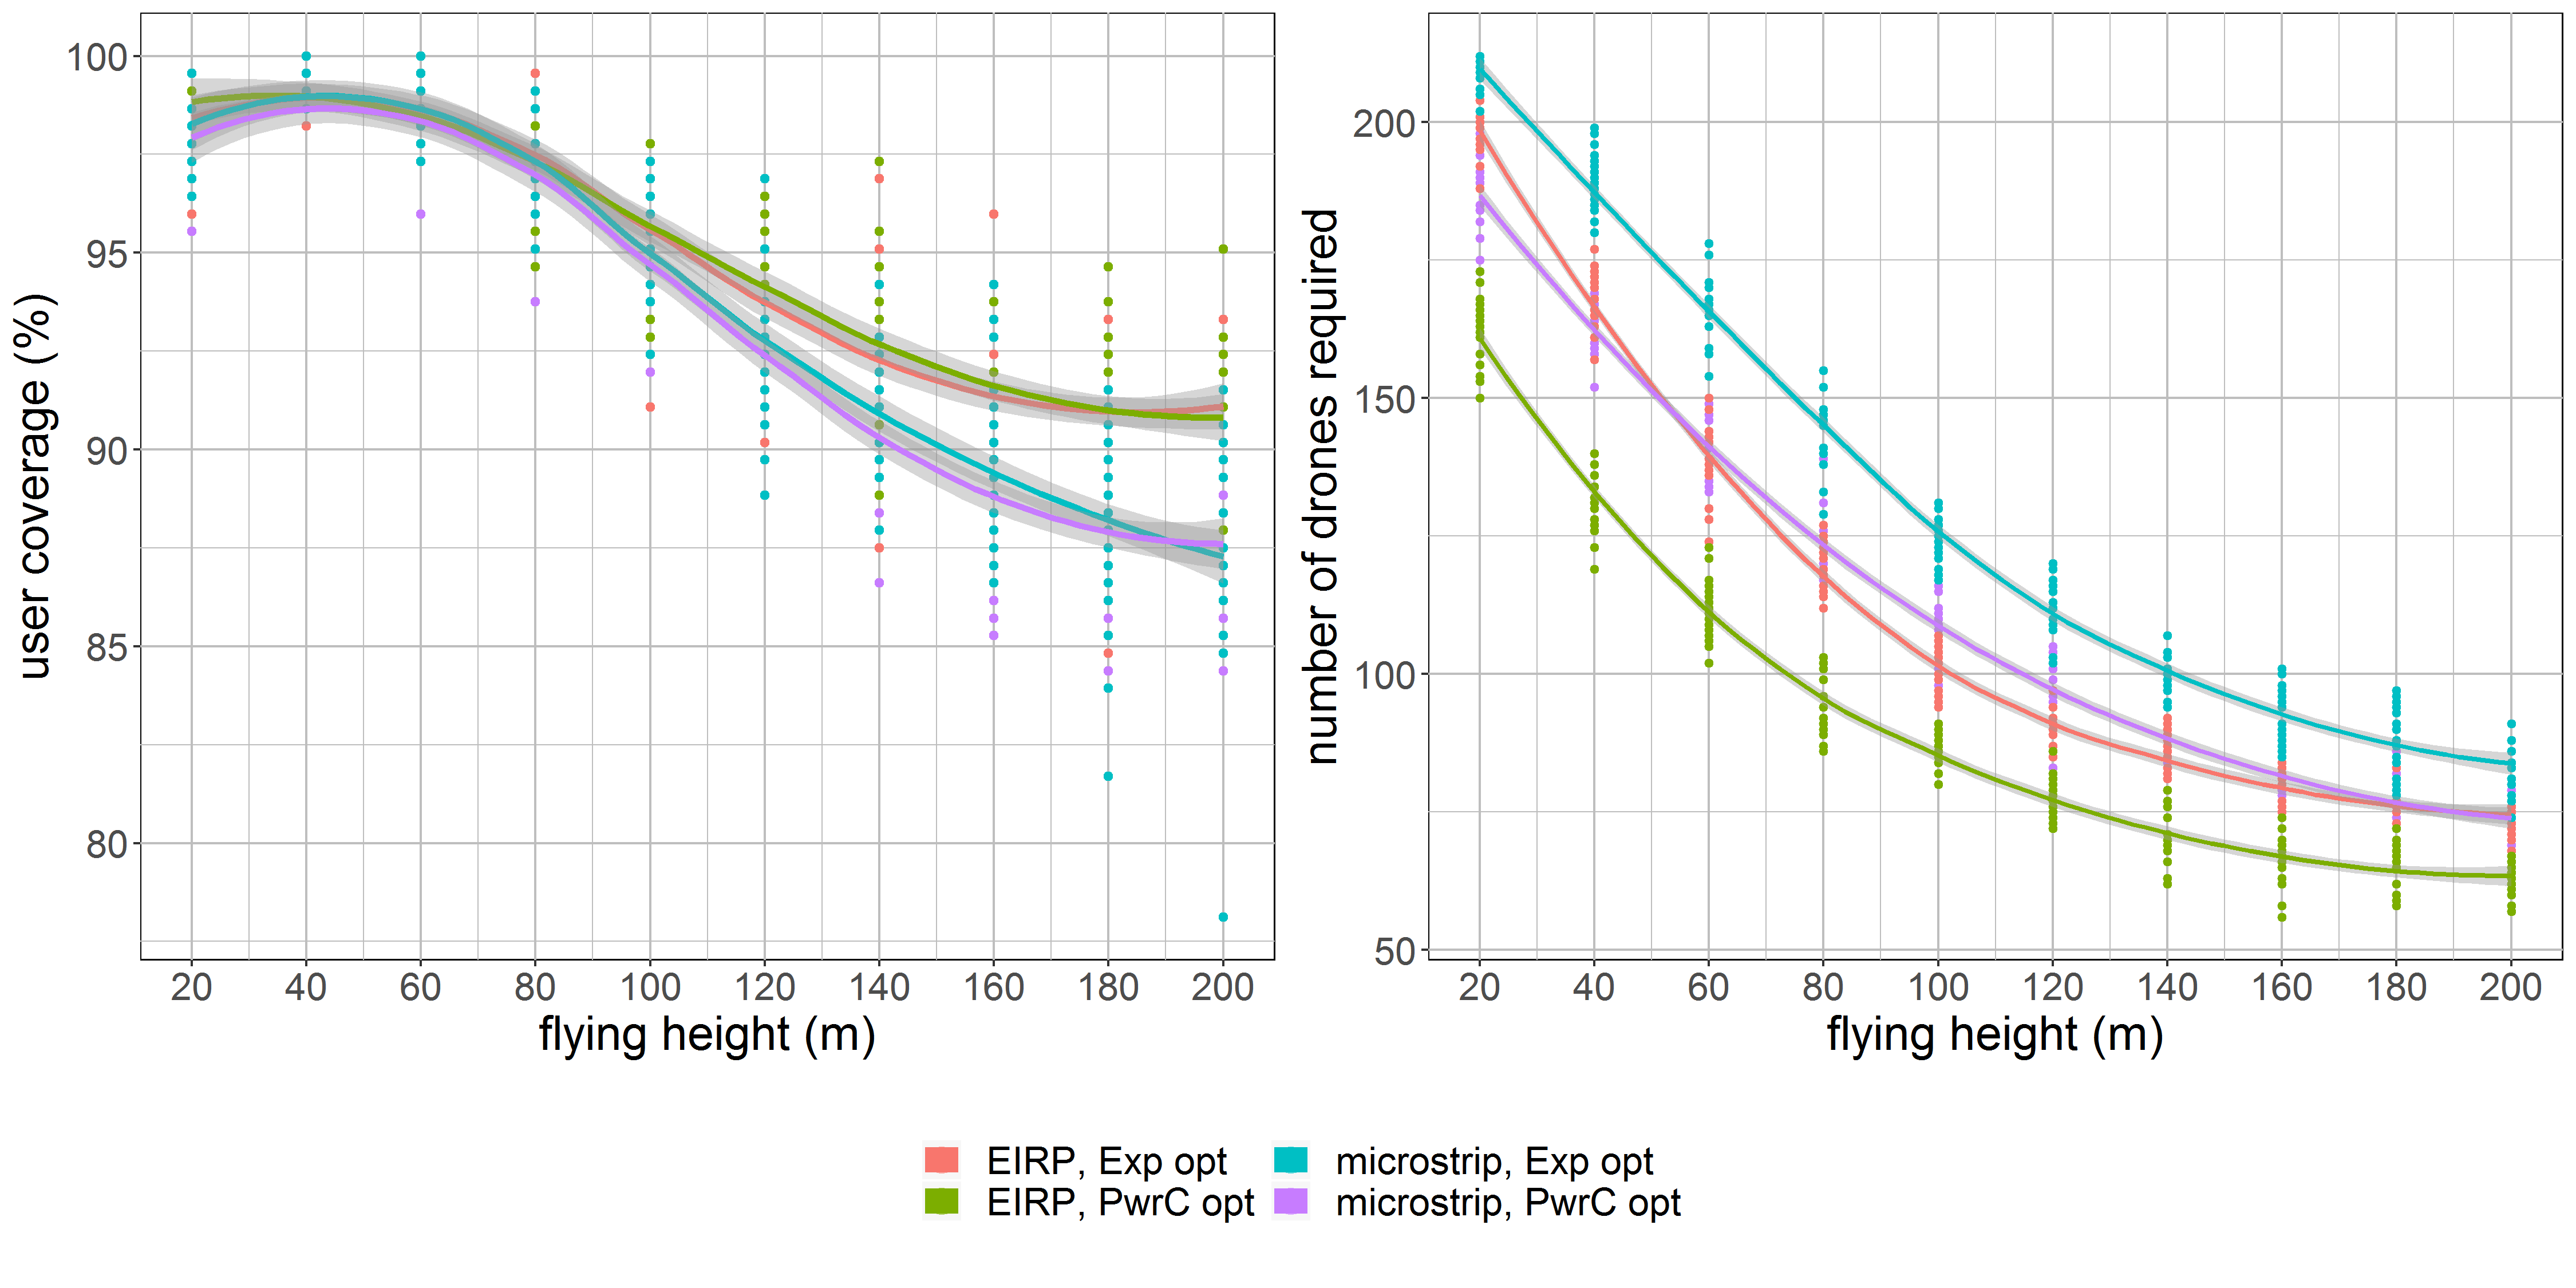
\includegraphics[width=\textwidth]{../results/s3/fhvsnumdronesAndCov.png}
  \caption{This graph shows how much \gls{UAV}s are required at different flying heights while trying to achieve a 100\% coverage.}
  \label{fig:s3a_numDronesAndCov}
\end{figure}

Both  \ref{fig:s3a_dlAndPc} and \ref{fig:s3a_numDronesAndCov} show that the network profits from increasing the flying altitude. 
Not only less \gls{UAV}s are needed but also the power consumption is lower. Both can be explained by the lower path loss when \gls{UABS}s fly higher.

Scenario 1 already proved that with low flying \gls{UAV}s, the main source of electromagnetic radiation are \gls{UABS}s. 
This changed around 80 meters where \gls{UL} electromagnetic radiation of the \gls{UE}
exceeds \gls{DL} radiation in order to still be able to reach the high flying \gls{UABS}s. 
When looking at the different individual sources in \ref{fig:s3a_fourSourcesMatrix}, we notice the same behaviour where the 
 \gls{UL} \gls{SAR} indeed increases. However, a more logarithmic increase is shown
  despite the fact that figure \ref{fig:s1_fhsar} showed that the  \gls{UL} \gls{SAR} 
increases exponentially. This was however deducted with only one user present in the network as opposed to this scenario 
where 224 users are present. The covered users will still behave like in scenario 1 but much more users are uncovered (fig. \ref{fig:s3a_numDronesAndCov}) 
which decreases the average \gls{SAR}. 
In conclusion, the average  \gls{UL} \gls{SAR}  will not increase as fast as the \gls{UL} \gls{SAR} of 
an individual that is covered.

\begin{figure}[]
  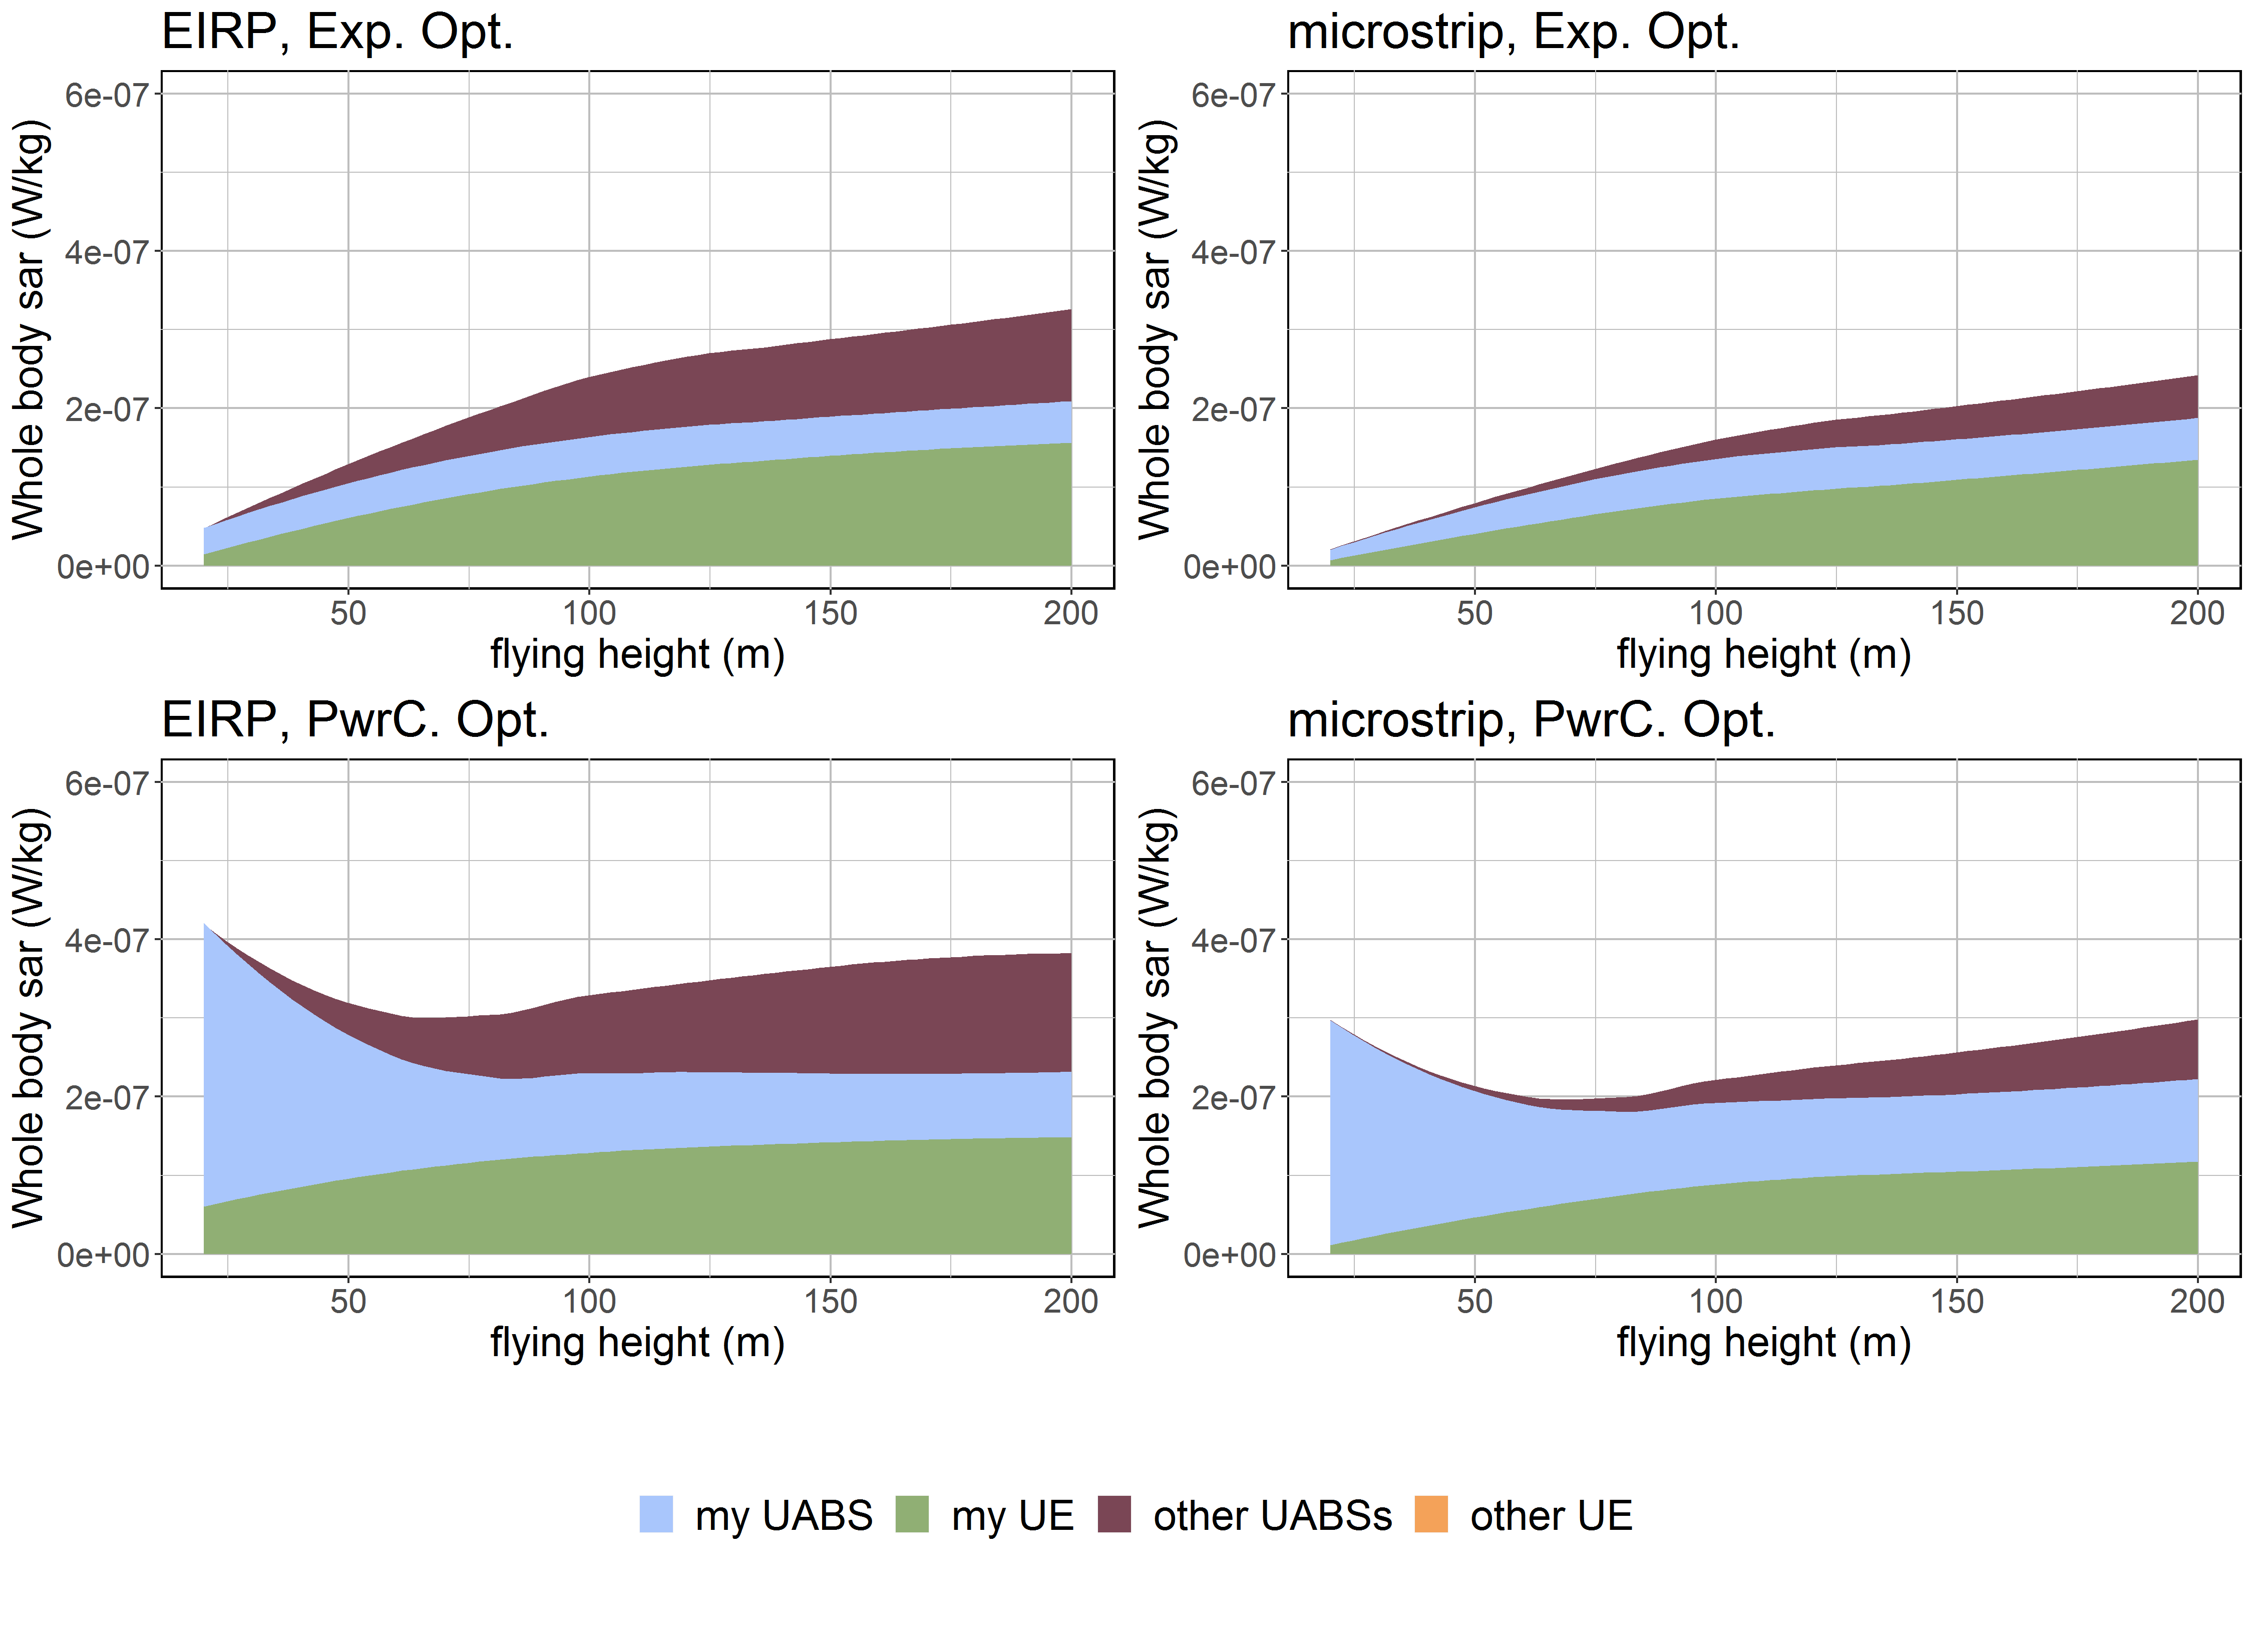
\includegraphics[width=\textwidth]{../results/s3/fhFourSources.png}
  \caption{
  Each figure corresponds with a certain configuration and shows how the \gls{SAR} from different sources are influenced by an increasing flying height.}  
  \label{fig:s3a_fourSourcesMatrix}
\end{figure}

We can see from \ref{fig:s3a_fourSourcesMatrix} that once out of the buildings level (around 70 to 80 meters), the SAR from the serving \gls{UABS} remains 
more or less constant. A behaviour that was already determined in `scenario 1' and `scenario 2: experiment \ref{fig:uvsulsarcentralUsers}'. 

When looking at the exposure from `other \gls{UABS}s', we see an increase in electromagnetic radiation at higher 
flying altitudes.
Also here the lower path loss from less obstructing buildings will be the reason.
The figures from \ref{fig:s3a_fourSourcesMatrix} further also clearly show that this increase 
in electromagnetic radiation will be less for a microstrip patch antenna. The reason behind this is that energy 
will be more focussed towards the ground and there is less sideways radiation because of attenuation.


%%%%%%%%%%%%%%%%%%%%%%%%%%%%%%%%%%%%%%%%%%%%%%%%%%%%%%%%%%%%%%%%%%%%%%%%%%%%%
\FloatBarrier
\subsection{Influence of the Number of Users}
\label{S3B}

The last case of scenario 3 investigates a variable number of users for a fixed flying height of 100 meters. There is no 
restriction on the number of available \gls{UAV}s just like in the previous case meaning that there are at most 
as much \gls{UAV}s as users in the network. The correct behaviour of the decision algorithm became already clear in the previous subsection \ref{S3A} but is also
confirmed by this case.
Figure \ref{fig:s3b_numdronesAndCov} shows on the left how the tool tries to reach a 100\% coverage. The tool reaches this goal 
better for larger populations. The difference remains however very little. The tool also requires more \gls{UAV}s for these large 
populations. An expected behaviour  when looking at scenario \ref{s2b} where, with only one \gls{UABS} available, the percentage of covered users decreases for these larger populations.
 The difference in optimization strategy is very little for small amounts of people but increases very quickly. Further, \ref{fig:s3b_dlAndPC} shows an increase 
 in exposure for larger populations because more \gls{UAV}s come with these larger populations and more 
 exposure comes with more \gls{UAV}s as visible in \ref{fig:s3b_numdronesAndCov}.

\begin{figure}[h!]
  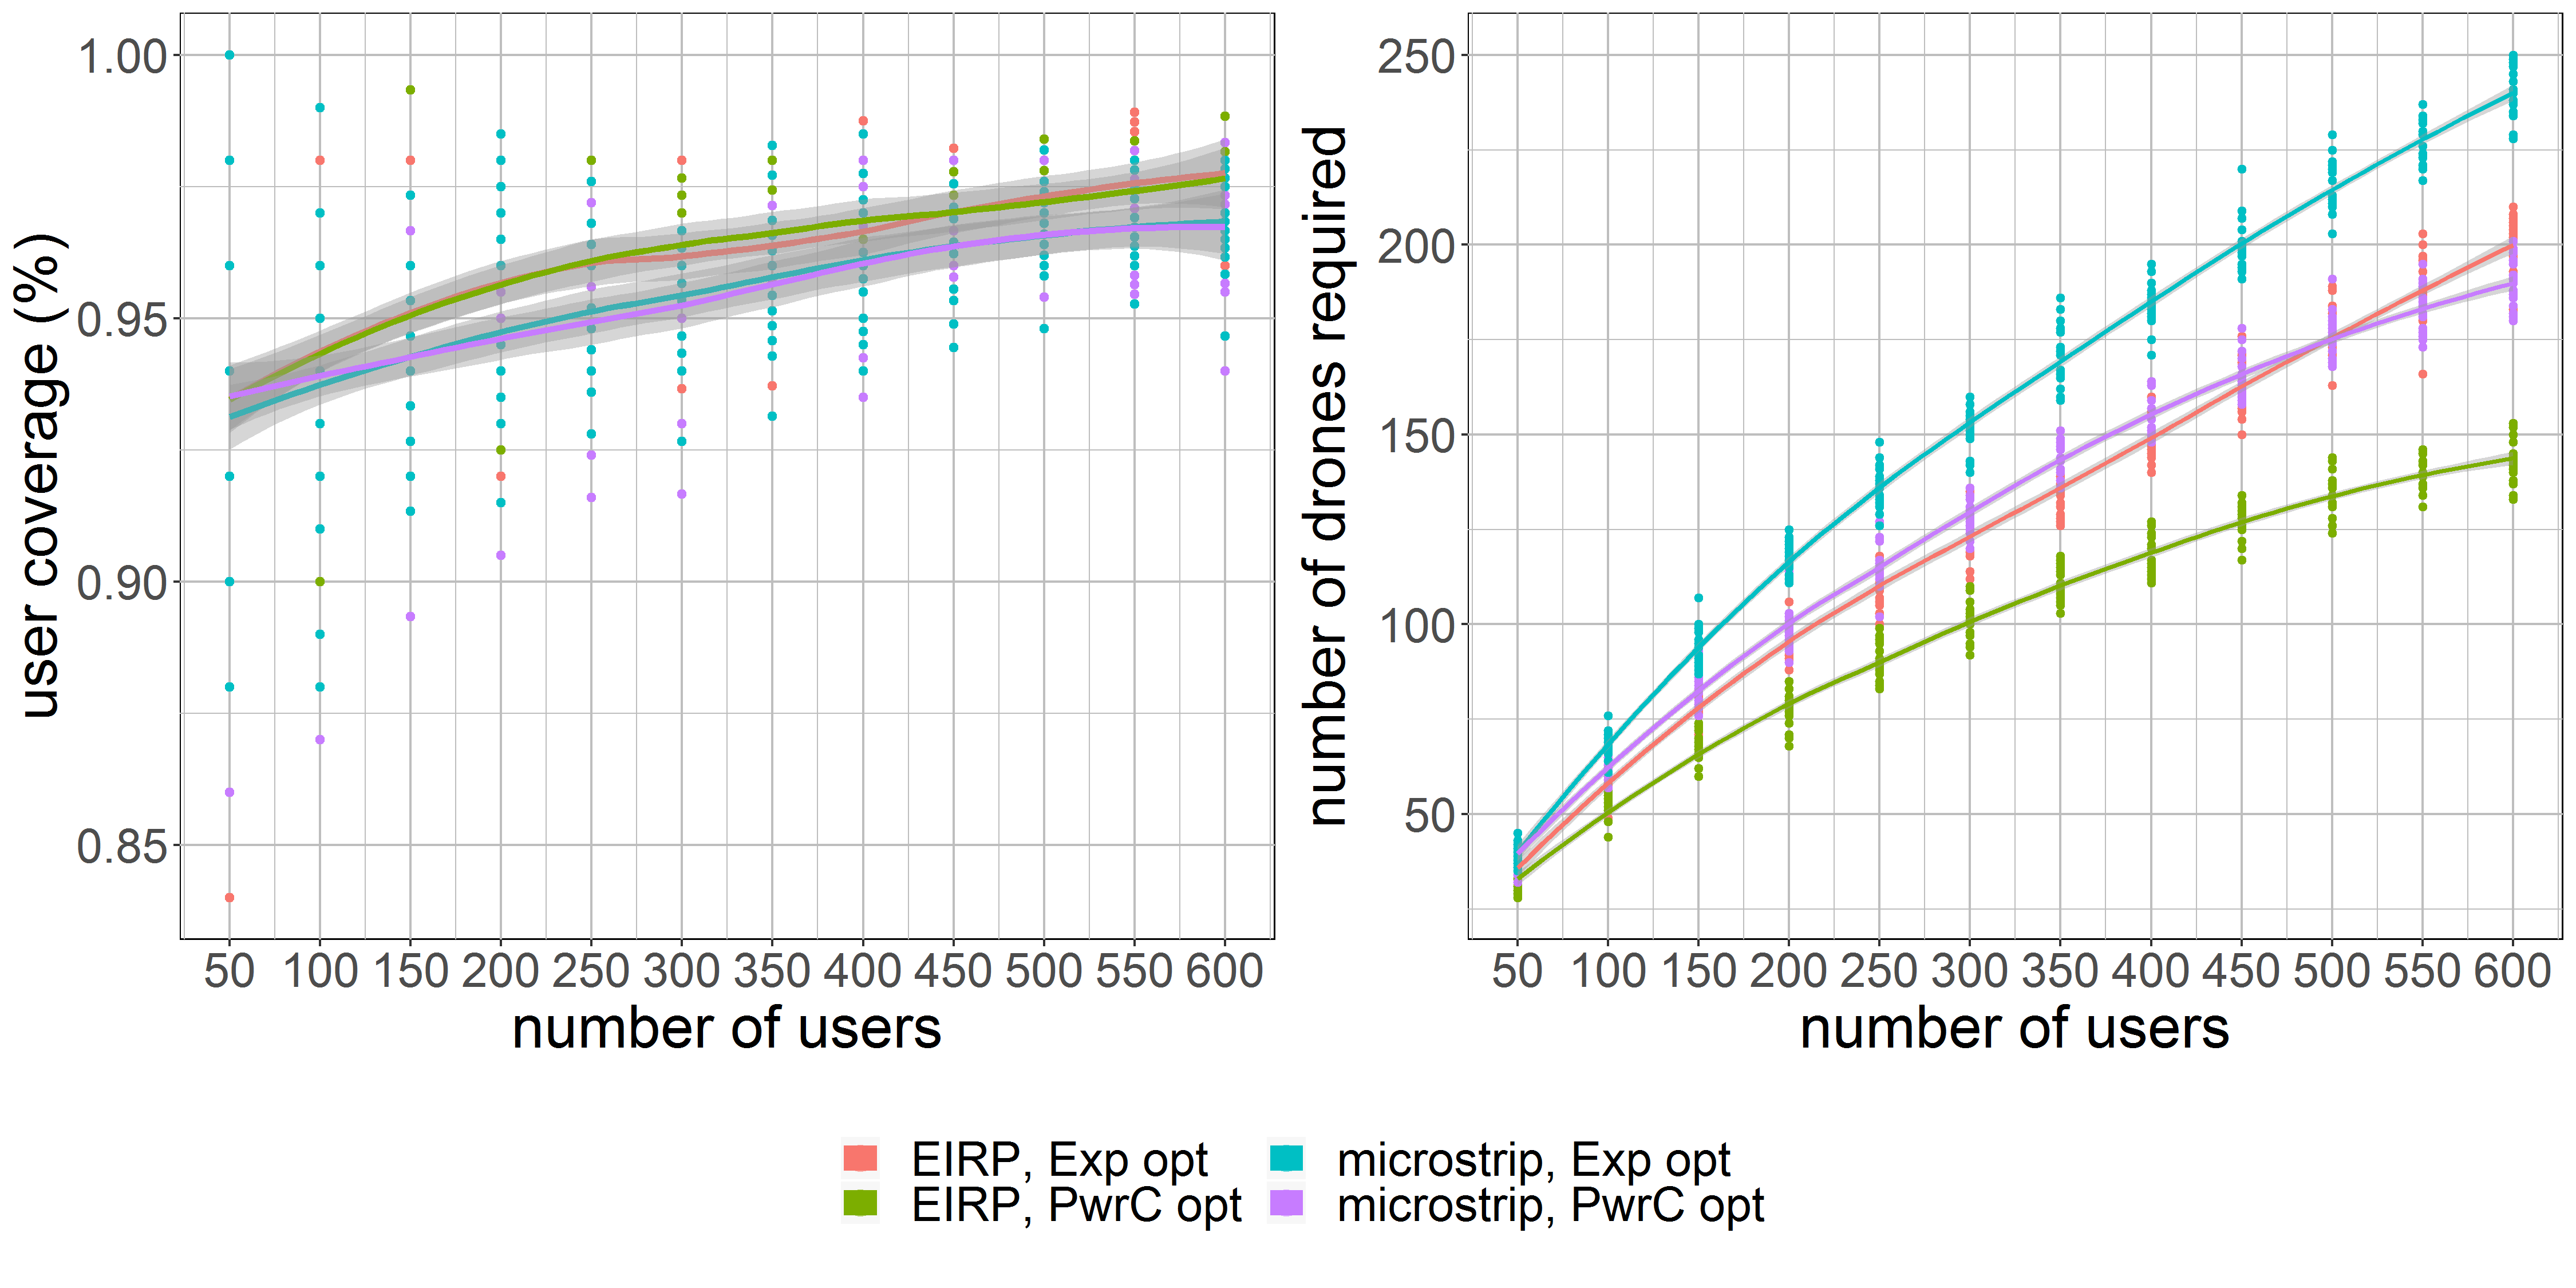
\includegraphics[width=\textwidth]{../results/s3/uvsnumdronesAndCov.png}
  \caption{This graph shows how much \gls{UAV}s are required for different flying heights while trying to achieve a 100\% coverage.}
  \label{fig:s3b_numdronesAndCov}
\end{figure}

In a scenario with 600 active users, a clear difference is noticeable between the four configurations. 
For instance, an EIRP power consumption optimized 
network requires the least amount of \gls{UAV}s (Figure \ref{fig:s3b_numdronesAndCov} on the right). This is logical when looking at figure \ref{fig:s3b_dlAndPC} where \gls{UAV}s in such a configuration cause 
the highest amount of 
electromagnetic radiation. This behaviour was already discussed in subsection \ref{s2b}. 

On the complete opposite, we have a microstrip patch antenna in an exposure optimized network. 
This strategy prioritizes the minimization of electromagnetic exposure. In addition, a microstrip antenna has a much more limited range.
Therefore, much more 
\gls{UAV}s are required in order to reach 100\% coverage (Figure \ref{fig:s3b_numdronesAndCov}) and therefore require much more energy 
to power all the \gls{UAV}s (Figure \ref{fig:s3b_numdronesAndCov} on the right).

This means that scenario 3 learns that a power consumption optimized network indeed results in less \gls{UAV}s and less 
 power consumption of the entire network. 
At the same time, scenario 2 showed that the active \gls{UABS}s have a higher individual power consumption.
We can therefore state that a power consumption optimized network will reduce its total power consumption by
using a few high powered \gls{UAV}s.

Likewise for an exposure optimized network, we can conclude that the network has indeed a lower electromagnetic exposure but the power consumption 
of the entire network is much higher. In scenario 2 became already clear that the active \gls{UABS}s have a low power consumption in order to 
guarantee a low electromagnetic exposure towards the users.
We can conclude that an exposure optimized network will reduce the exposure of an individual by 
using a lot of low powered \gls{UAV}s.

\begin{figure}[h!]
  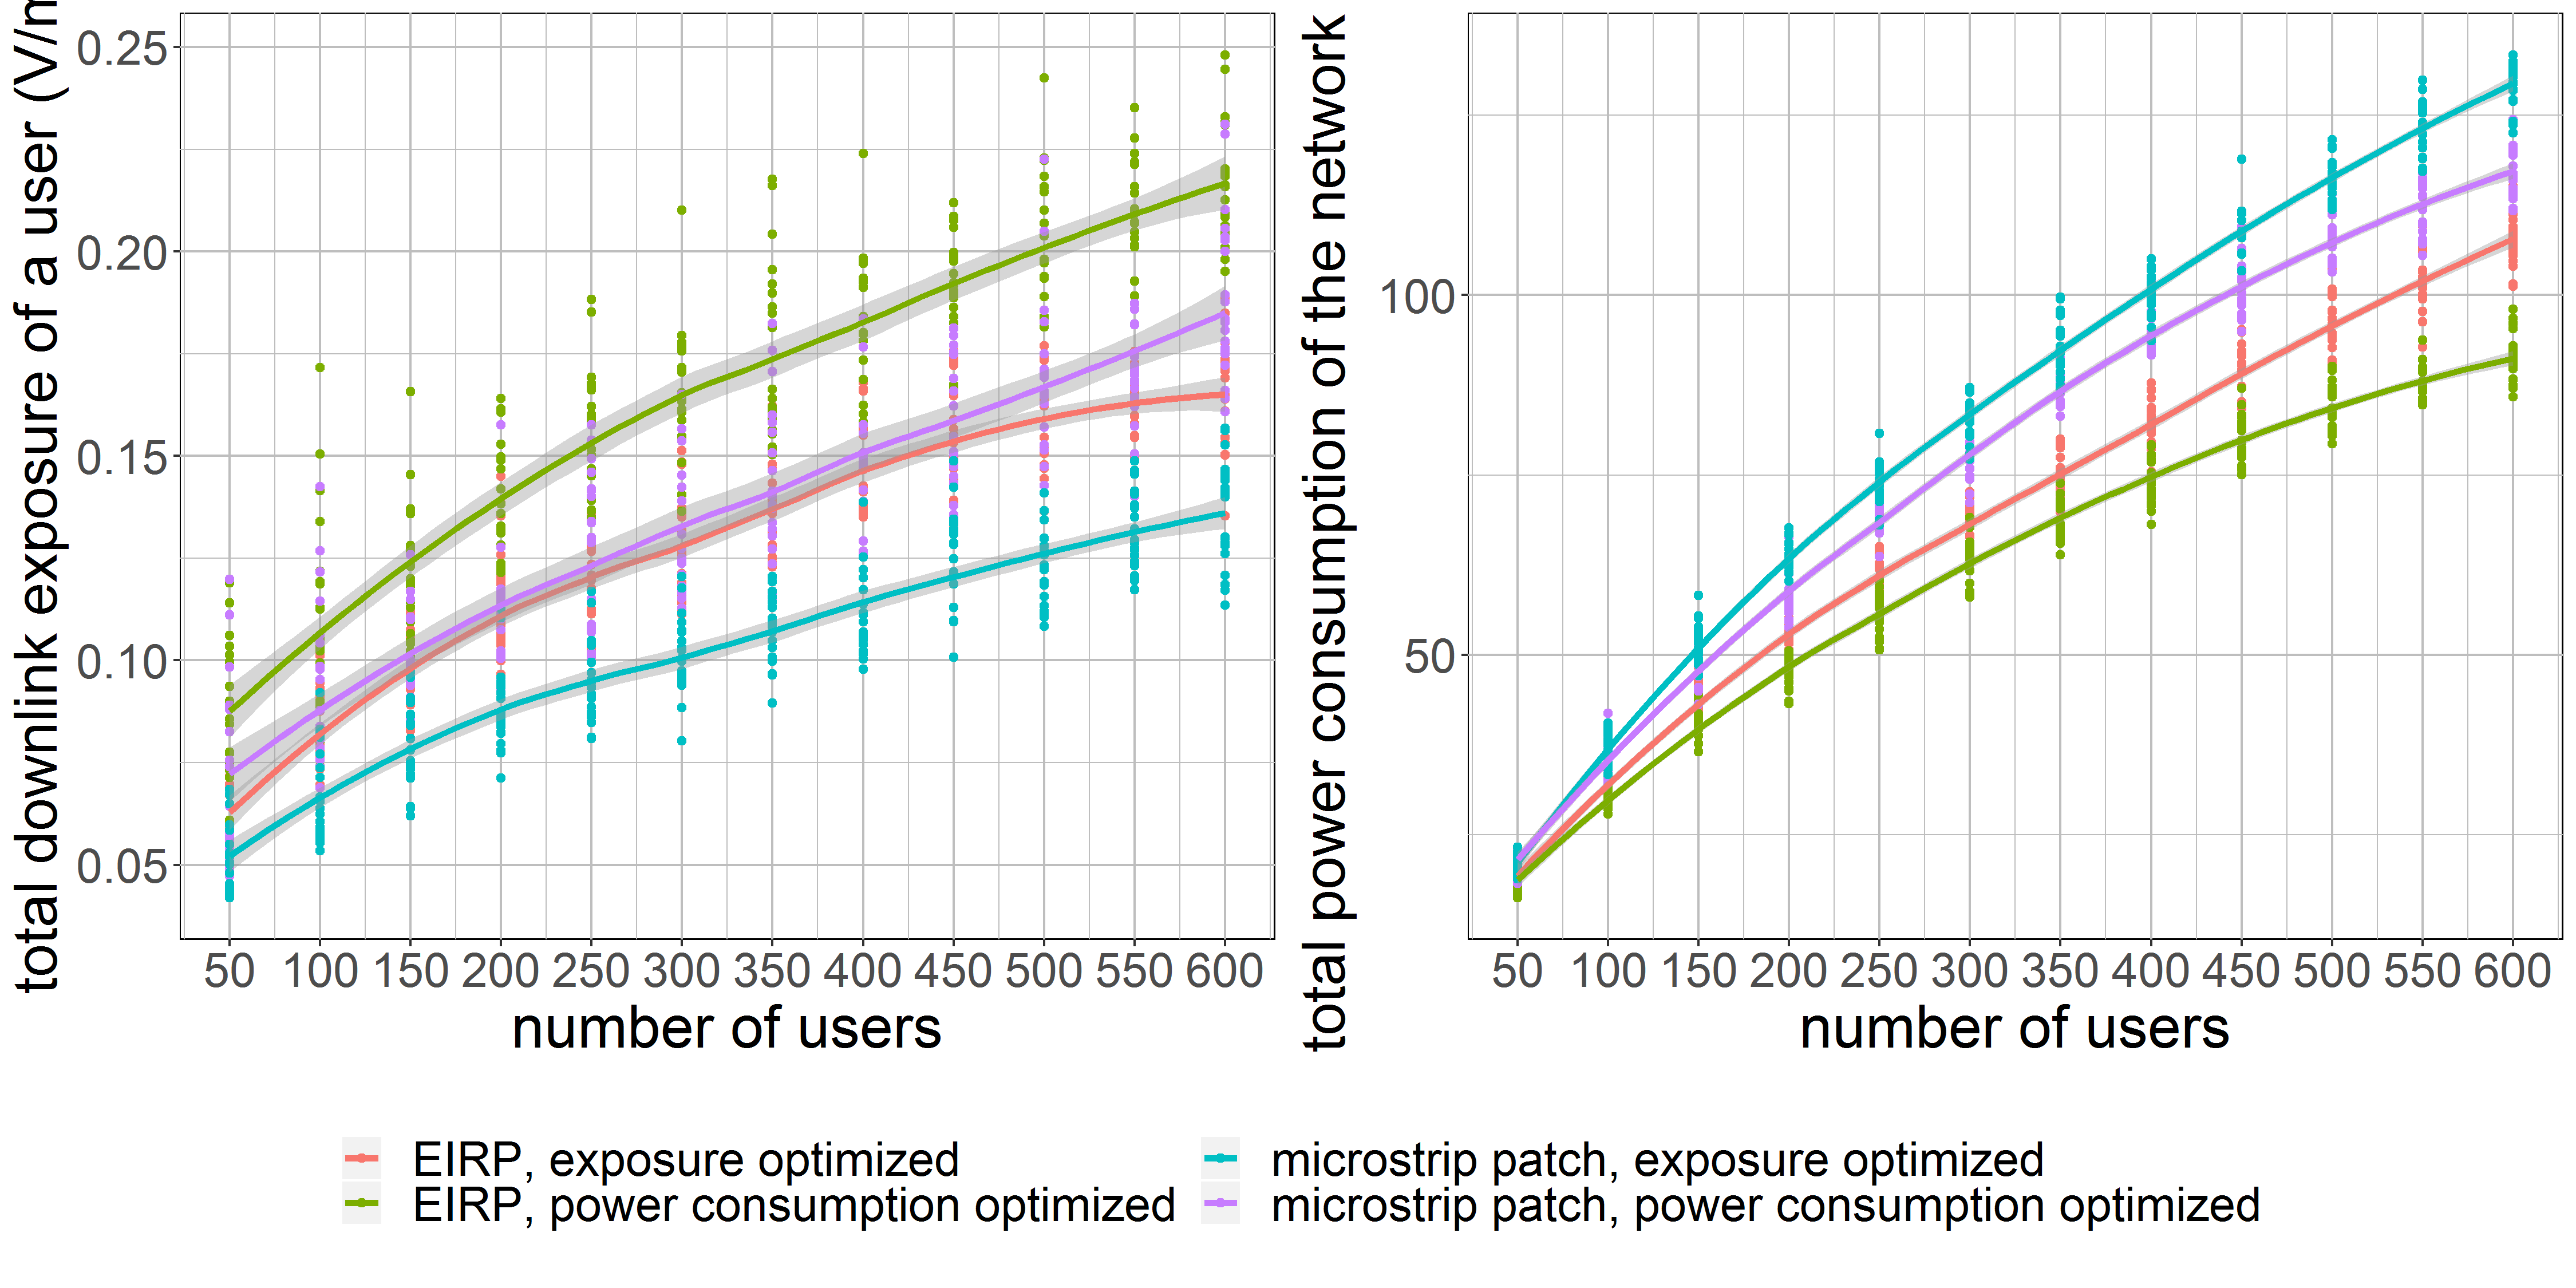
\includegraphics[width=\textwidth]{../results/s3/uvsdlAndPc.png}
  \caption{The influence of the population density on the downlink electromagnetic radiation (left) and power consumption (right).}
  \label{fig:s3b_dlAndPC}
\end{figure}

When looking at the different contributions to the total \gls{SAR} in figure \ref{fig:s3b_fourSourcesMatrix}, 
we see that the weighted average 
\gls{SAR} from the users own device and from the serving \gls{UABS} remains constant. The flying altitude is always the same so 
also the required energy to cover that distance will remain the same. 
The only \gls{SAR} value that increases are the \gls{DL} \gls{SAR} from other \gls{UABS}s and the \gls{UL} \gls{SAR} from other \gls{UE}. 
When more users come online, also more \gls{UAV}s will be radiating. Moreover, there is very little path loss because the flying height is above the average building.

\begin{figure}[h!]
  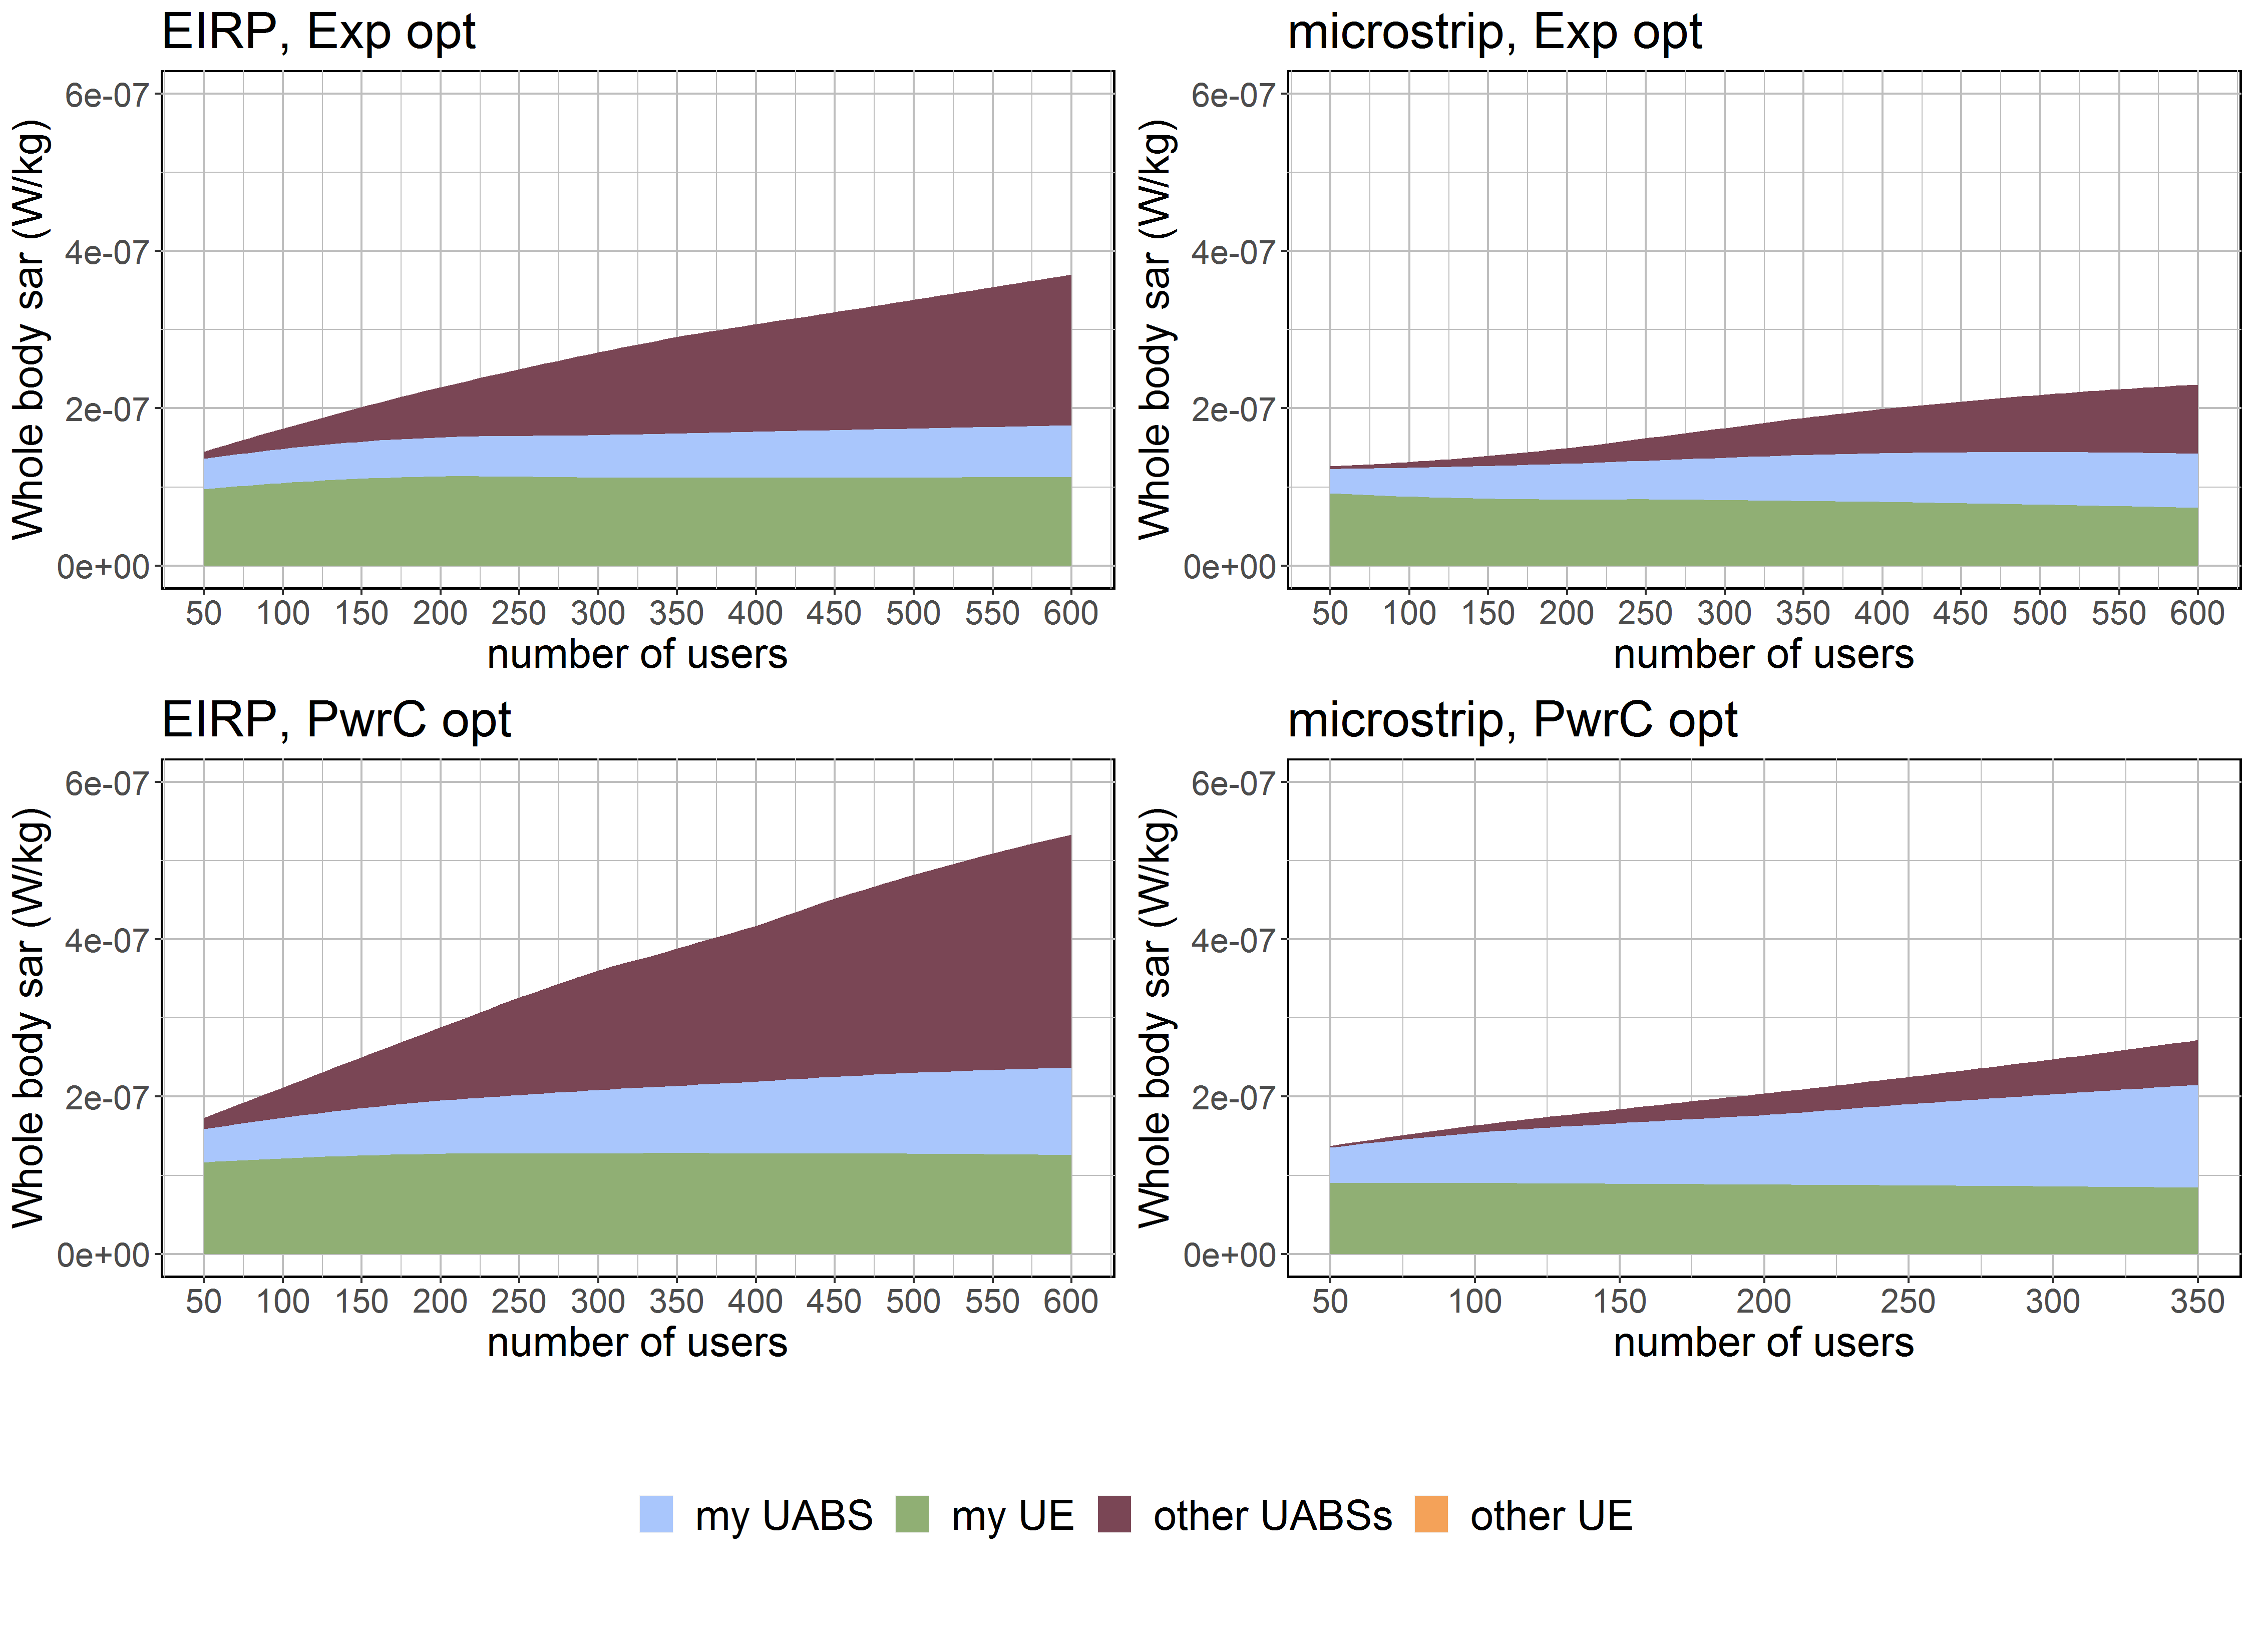
\includegraphics[width=\textwidth]{../results/s3/uFourSources.png}
  \caption{Each figure corresponds with a certain configuration and shows how the \gls{SAR} 
  from different sources are influenced by an increasing population density. Unlimited number of \gls{UABS} are available.
  }
  \label{fig:s3b_fourSourcesMatrix}
\end{figure}